%%%%%%%%%%%%%%%%%%%%%%%%%%%%%%%%%%%%%%%%%%%%%%%
% Template baseado no exemplo da classe utftex
% Prof. César M. V. Benítez
% DAELN, UTFPR-Curitiba (2019)
%%%%%%%%%%%%%%%%%%%%%%%%%%%%%%%%%%%%%%%%%%%%%%%


\documentclass[openright]{normas-utf-tex} %openright = o capitulo comeca sempre em paginas impares
%\documentclass[oneside]{normas-utf-tex} %oneside = para numero de paginas menor que 100 (apenas frente da folha) 

% force A4 paper format
\special{papersize=210mm,297mm}

\usepackage[alf,abnt-emphasize=bf,bibjustif,recuo=0cm, abnt-etal-cite=2, abnt-etal-list=99]{abntcite} %configuracao correta das referencias bibliograficas.

\usepackage[portuguese, ruled, linesnumbered]{algorithm2e}%pacotedealgoritmoemportugues

\usepackage[brazil]{babel} % pacote portugues brasileiro
\usepackage[utf8]{inputenc} % pacote para acentuacao direta
\usepackage{amsmath,amsfonts,amssymb} % pacote matematico
\usepackage{graphicx} % pacote grafico
\usepackage{times} % fonte times
\usepackage[final]{pdfpages} % adicao da ata
\usepackage[version=3]{mhchem}%adição de pacote para quimica
\usepackage{longtable}% redimensionar automaticamente tabelas
%\usepackage{hyperref}% link das res
\newcommand\tab[1][1cm]{\hspace*{#1}}
%Podem utilizar GEOMETRY{...} para realizar pequenos ajustes das margens. Onde, left=esquerda, right=direita, top=superior, bottom=inferior. P.ex.:
%\geometry{left=3.0cm,right=1.5cm,top=4cm,bottom=1cm} 
\usepackage{amsthm}
\newtheorem{mydef}{Definicão}

%\usepackage{balance} 



% ---------- Preambulo ----------
\instituicao{ UNIVERSIDADE TECNOLÓGICA FEDERAL DO PARANÁ (UTFPR)} % nome da instituicao
\programa{Curso de Engenharia de Computação} % nome do programa
\area{Engenharia de Computação} 
\documento{Oficina de Integração 2 -- Relatório Final} % Oficina de Integração 1 ou 2
\nivel{Graduação em Engenharia de Computação} 
\titulacao{Graduação em Engenharia de Computação} 

\titulo{Projeto GoBike} % titulo do trabalho em portugues
\title{\MakeUppercase{GoBike Project}} % titulo do trabalho em ingles

\autor{Frank Edmundo Huscher Bloemer \protect \\ João Lucas Mizuguchi Ferreira \\ \protect Thiago Ramos Bernardo} % autor do trabalho
%\cita{aluno1} % sobrenome (maiusculas), nome do autor do trabalho


\palavraschave{Ciclismo; Tecnologia; Rastreio; Segurança}  % palavras-chave do trabalho
\keywords{Cycling; Technology; Tracking; Safety} % palavras-chave do trabalho em ingles

\comentario{Relatório Final da disciplina Oficina de Integração 2,  % Oficina de integração 1 ou 2 
do curso de Engenharia de Computação, 
apresentado aos professores que ministram a 
mesma na Universidade Tecnologica Federal do 
Paraná como requisito parcial para obtenção da 
aprovação na disciplina.} 

\orientador{Prof. Dr. César Manuel Vargas Benítez \protect \\ 
Prof. Dr. Daniel Rossato} % nome do orientador do trabalho



\local{Curitiba} % cidade
\data{\the\year} % ano automatico

% desativa hifenizacao mantendo o texto justificado.
% thanks to Emilio C. G. Wille
\tolerance=1
\emergencystretch=\maxdimen
\hyphenpenalty=10000
\hbadness=10000
\sloppy

%---------- Inicio do Documento ----------
\begin{document}

\capa % geracao automatica da capa
\folhaderosto % geracao automatica da folha de rosto


% % dedicatoria (opcional)
\begin{dedicatoria}
% Texto da dedicat\'oria.
Este trabalho é dedicado especialmente a nossas famílias, sem as quais nada disso seria possível.

\end{dedicatoria}

% % agradecimentos (opcional)
\begin{agradecimentos}
% Texto dos agradecimentos.
Primeiramente, gostaríamos de agradecer a Deus pelas conquistas e bênçãos obtidas. Gostaríamos também de agradecer a nossas famílias e amigos, que nos motivaram, apoiaram e deram forças em todos os momentos em que mais precisamos. Por fim, somos imensamente gratos ao Sr. Rafael Juliani pela grande ajuda com a modelagem e impressão 3D presentes neste projeto.

 \end{agradecimentos}

% % epigrafe (opcional)
% \begin{epigrafe}
% Texto da ep\'igrafe.
% \end{epigrafe}

%resumo
\begin{resumo}
Este documento descreve o Go Bike, projeto realizado para a disciplina de Oficina de Integracão 2. O projeto tem como objetivo a construção de um sistema que possibilite uma melhor segurança para os ciclistas e suas bicicletas. O sistema é composto por um módulo instalado na bicicleta e um aplicativo para celular, que juntos fornecem informações sobre a localização de bicicletas do usuário e amigos, sendo possível compartilhar essa localização com amigos, estacionar a bicicleta em algum lugar e receber alertas via notificação caso ela saia do lugar. O aplicativo é desenvolvido em Flutter para Android e o módulo é em um ESP32. Foram usadas diversas bibliotecas para o desenvolvimento do projeto, como o MongoDB para o banco de dados, o Firebase para as notificações, o Open Street Map para a localização no aplicativo. Ao final do projeto foi possível atingir o objetivo proposto, com o módulo instalado na bicicleta sendo capaz de enviar informações para o aplicativo e com o aplicativo sendo capaz de receber essas informações e exibi-las ao usuário.
\end{resumo}

%abstract
\begin{abstract}
This document describes Go Bike, a project carried out for the subject of Oficina de Integracão 2. The project aims to build a system that provides better safety for cyclists and their bicycles. The system consists of a module installed on the bike and a mobile application, which together provide information about the location of the user's bikes and friends, making it possible to share this location with friends, park the bike somewhere and receive alerts via notification if she leaves the place. The application is developed in Flutter for Android and the module is in an ESP32. Several libraries were used for the development of the project, such as MongoDB for the database, Firebase for notifications, Open Street Map for the location in the application. At the end of the project, it was possible to achieve the proposed objective, with the module installed on the bicycle being able to send information to the application and with the application being able to receive this information and display it to the user. At the end of the project, it was possible to achieve the proposed objective, with the module installed on the bicycle being able to send information to the application and with the application being able to receive this information and display it to the user.
\end{abstract}

% listas (opcionais, mas recomenda-se a partir de 5 elementos)
\listadefiguras % geracao automatica da lista de figuras
\listadetabelas % geracao automatica da lista de tabelas
%\listadequadros % adivinhe :)
%\listadesiglas % geracao automatica da lista de siglas
%\listadesimbolos % geracao automatica da lista de simbolos

% sumario
\sumario % geracao automatica do sumario


%---------- Inicio do Texto ----------
% recomenda-se a escrita de cada capitulo em um arquivo texto separado (exemplo: intro.tex, fund.tex, exper.tex, concl.tex, etc.) e a posterior inclusao dos mesmos no mestre do documento utilizando o comando \input{}, da seguinte forma:
%\input{intro.tex}
%\input{fund.tex}
%\input{exper.tex}
%\input{concl.tex}

% Colocar aqui o numero da página inicial!!! (Obs.: conta a partir da folha de rosto)
\setcounter{page}{12}



\chapter{Introdução}
Este projeto visa, em suma, trazer uma ampla gama de funcionalidades e praticidades para o ciclista, com baixo custo e sem que este necessite de seu celular durante a atividade.
\section{Motivação} %qual o problema?
Quando um ciclista sai para pedalar, muitas vezes não é prático e é até perigoso que ele leve o seu celular no bolso ou em um suporte na bicicleta, visto que pode derrubar o aparelho, se acidentar ou até mesmo ser roubado em um momento de distração ou descuido.
Tendo em mente esses problemas a ideia do GoBike foi concebida com o intuito de resolver esse problema, sendo um módulo que pode ser removível da bicicleta que será capaz de captar a velocidade e localização do usuário, e posteriormente trazer todas essas informações em um aplicativo.
\section{Objetivos}
\subsection{Objetivo geral} 
O objetivo da realização deste projeto é desenvolver um sistema integrado à bicicleta que possibilite acesso à um conjunto amplo de funções úteis para o ciclista, como a velocidade e compartilhamento de localização, sem que este precise carregar consigo o seu celular durante a atividade de pedalar, assim tornando a prática mais segura trazendo conforto para os amigos e familiares. 
\subsection{Objetivos específicos}
Construção de um dispositivo que consiga:
\begin{itemize}
  \item Ser removível da bicicleta.
  \item Verificar a velocidade através de uma tela na bicicleta.
  \item Rastrear a localização do módulo.
  \item Estacionar a bicicleta e entrar em modo de segurança.
  \item Enviar notificações para o aplicativo para avisar quando a bicicleta está saindo do modo de segurança.
  \item Enviar notificações para o aplicativo caso a bicicleta esteja saindo do lugar e avisar de possíveis roubos.
  \item Permitir o compartilhamento da localização do módulo com amigos e familiares através do aplicativo.
  \item Obter as direções do módulo através da última localização disponível.
\end{itemize}

\subsection{Requisitos}

\textbf {Requisitos Funcionais (RF)}
\begin{itemize}
  \item RF01 - O aplicativo deve permitir o rastreio da bicicleta do usuário, ser capaz de ativar o modo de estacionar, receber notificações quando em modo estacionar e ver a localização de bicicleta de amigos.
  \item RF02 - O equipamento deve ser capaz de medir a velocidade do usuário.
  \item RF03 - O software deve salvar a posição do usuário.
  \item RF04 - O software deve se conectar ao celular via bluetooth.
  \item RF05 - O sistema deve possuir conexão com a internet via chip (SIM).
  \item RF06 - O hardware deve possuir um display para visualizar as informações.
  \item RF07 - A tela deve exibir a temperatura, atualizada de tempos em tempos.
  \item RF08 - A parte mecânica deve estar acoplada na bicicleta, estrutura demonstrada na Figura 4.
  \item RF09 - O software deve registrar as informações em um banco de dados.
  \item RF10 - O sistema deve possuir um botão para estacionar a bicicleta.
\end{itemize}
\newpage
\textbf {Requisitos Não-Funcionais (RNF)}
\begin{itemize}
  \item RNF01 - O app deve ser compatível com Android.
  \item RNF02 - A bateria deve durar 20 minutos.
  \item RNF03 - A parte mecânica deve permanecer estável enquanto o usuário pedala.
  \item RNF04 - O sistema deve ser removível.
  \item RNF05 - O sistema deve minimizar o consumo de internet.
\end{itemize}
   %Introducao
\chapter{Fundamentação teórica}
Com relação a fundamentação teórica do projeto, foram agrupados estudos sobre as tecnologias utilizadas no projeto a fim de quais delas era a mais recomendada para o escopo do projeto. Além disso, foram analizados vídeos, tutoriais e blogs com exemplos e aplicações dos componentes comprados [3], além de leituras minuciosas dos datasheets dos componentes utilizados [4], a fim de conhecer suas principais funcionalidades, requisitos e particularidades.

\section{ESP32}
O ESP32 é um microcontrolador de 32 bits com Wi-Fi e Bluetooth integrados, desenvolvido pela Espressif Systems. Ele é baseado no processador Tensilica Xtensa LX6 dual-core, com 2 núcleos de processamento, que opera a 240 MHz. Possui 520 KB de RAM e 4 MB de memória flash, além de suporte a Wi-Fi 802.11 b/g/n, Bluetooth 4.2 BR / EDR e BLE, além de capacidade de transmissão de dados de 150 Mbps e consumo de energia extremamente baixo. O ESP32 também possui uma porta USB OTG, que permite que ele seja conectado a um computador ou a um dispositivo móvel, o que o torna uma boa alternativa para o desenvolvimento de dispositivos IoT.

\section{OLED}
OLED é um tipo de display de cristal líquido que utiliza um painel de cristal líquido orgânico (OLED) para produzir imagens. Um OLED é formado por uma matriz de pixels que são controlados individualmente por um circuito integrado. Cada pixel pode ser desligado, ligado ou variar a intensidade da luz emitida, o que permite que a imagem seja exibida em preto e branco ou colorida. No projeto foi utilizado para apresentar a velocidade do usuário e feedbacks sobre a conexão MQTT do módulo.

\section{GSM GPRS SIM800L}
O SIM800L é um módulo GSM/GPRS de baixo custo que pode ser usado para comunicação de dados, chamadas telefônicas e SMS. O SIM800L é baseado no módulo SIM800C e possui um microcontrolador incorporado, que pode ser usado para enviar e receber mensagens SMS, fazer e receber chamadas telefônicas, enviar e receber dados, etc. No projeto foi inicialmente utilizado para atuar como \textit{hotspot} de internet do módulo.

\section{GPS GY-NEO6MV2}
O módulo GPS GY-NEO6MV2 é uma placa compacta indicada para projetos de navegação aérea ou terrestre com a finalidade de definir a geolocalização e fornecer os dados para uma plataforma microcontrolada, ela possui uma comunicação serial/TTL de 2 pinos (RX e TX) de 9600bps, funciona com 3.3V à 5V, possui uma antena embutida e tem precisão de 5m. A sua função no projeto é captar os valores da latitude, longitude e velocidade.

\section{MPU6050}
O MPU6050 é um sensor de aceleração e giroscópio de 6 eixos que fornece 9 eixos de medição (3 eixos de aceleração e 3 eixos de giroscópio) com um único sensor. No projeto foi utilizado para verificar se houve movimento enquanto a bicicleta está estacionada.

\section{Flutter}
Flutter é um kit de ferramentas de código aberto criado pelo Google. Ele é usado para desenvolver aplicativos para Android e iOS. Flutter usa o Dart como sua linguagem de programação principal. O Dart é uma linguagem de programação orientada a objetos desenvolvida pelo Google. Ele é compilado em código nativo e foi utilizado para desenvolver o aplicativo Go Bike em Android.

\section{Firebase}
Firebase é uma plataforma de desenvolvimento de aplicativos móveis e da Web, fornecida pela Google. Ele fornece recursos de armazenamento de dados, banco de dados, autenticação, mensagens em tempo real, notificações, análise e muito mais. O Firebase é usado para desenvolver aplicativos móveis e da Web modernos e escaláveis. No projeto foi utilizado o Firebase para enviar as notificações para o aplicativo. O aplicativo desenvolvido nesse projeto foi testado apenas em Android.

\section{MongoDB}
MongoDB é um banco de dados NoSQL orientado a documentos. Os documentos são armazenados em coleções, que são semelhantes a tabelas em um banco de dados relacional. Um documento é uma estrutura de dados que pode ser armazenada no MongoDB. Ele é composto por campos, que são agrupados em pares de chave-valor. Os documentos são semelhantes a objetos JSON. Foi utilizado para salvar as localizações do módulo Go Bike, contendo latitude, longitude e velocidade.

\section{MQTT}
MQTT é um protocolo de comunicação leve e de código aberto que pode ser usado para construir sistemas de Internet das Coisas (IoT). O MQTT é um protocolo de mensagens publicadas / assinadas, que significa que um cliente pode publicar uma mensagem em um tópico, e todos os clientes assinados para esse tópico receberão a mensagem. O MQTT é baseado em TCP / IP e usa o protocolo TCP para enviar mensagens. Foi utilizado no projeto para a comunicação entre o ESP32 e a API.

\section{HTTP}
O protocolo de transferência de hipertexto (HTTP) é um protocolo de aplicação de camada de apresentação usado para comunicação de dados entre clientes e servidores. Ele é usado para transferir documentos HTML, imagens, arquivos de vídeo, etc. entre um cliente e um servidor. O HTTP é baseado em solicitação / resposta. Foi utilizado no projeto para a comunicação entre o aplicativo e a API.   %Fundamentacao teorica
\chapter{Metodologia}
A metodologia deste trabalho envolve desenvolver e aplicar conceitos e conhecimentos de hardware, software e mecânica. Alguns destes conhecimentos a equipe já possuía anteriormente, mas a grande maioria precisou ser desenvolvida com o decorrer do trabalho.
\section{Visão geral}
Na Figura \ref{fig:diagrama_hardware} é possivel observar o diagrama geral do projeto com todos os seus componentes principais e as suas funções, o ESP32 tem a função de controlador geral do projeto, ele controla o GSM e OLED, lê os dados dos sensores e se comunica com o MQTT, o GPS capta a latitude, a longitude e a velocidade, o acelerômetro capta a aceleração, o OLED exibe a velocidade, o GSM age como um hotspot 2G para o ESP32 e o MQTT age como uma ponte para a conexão entre o aplicativo e o ESP32.

\begin{figure}[!h]
\centering
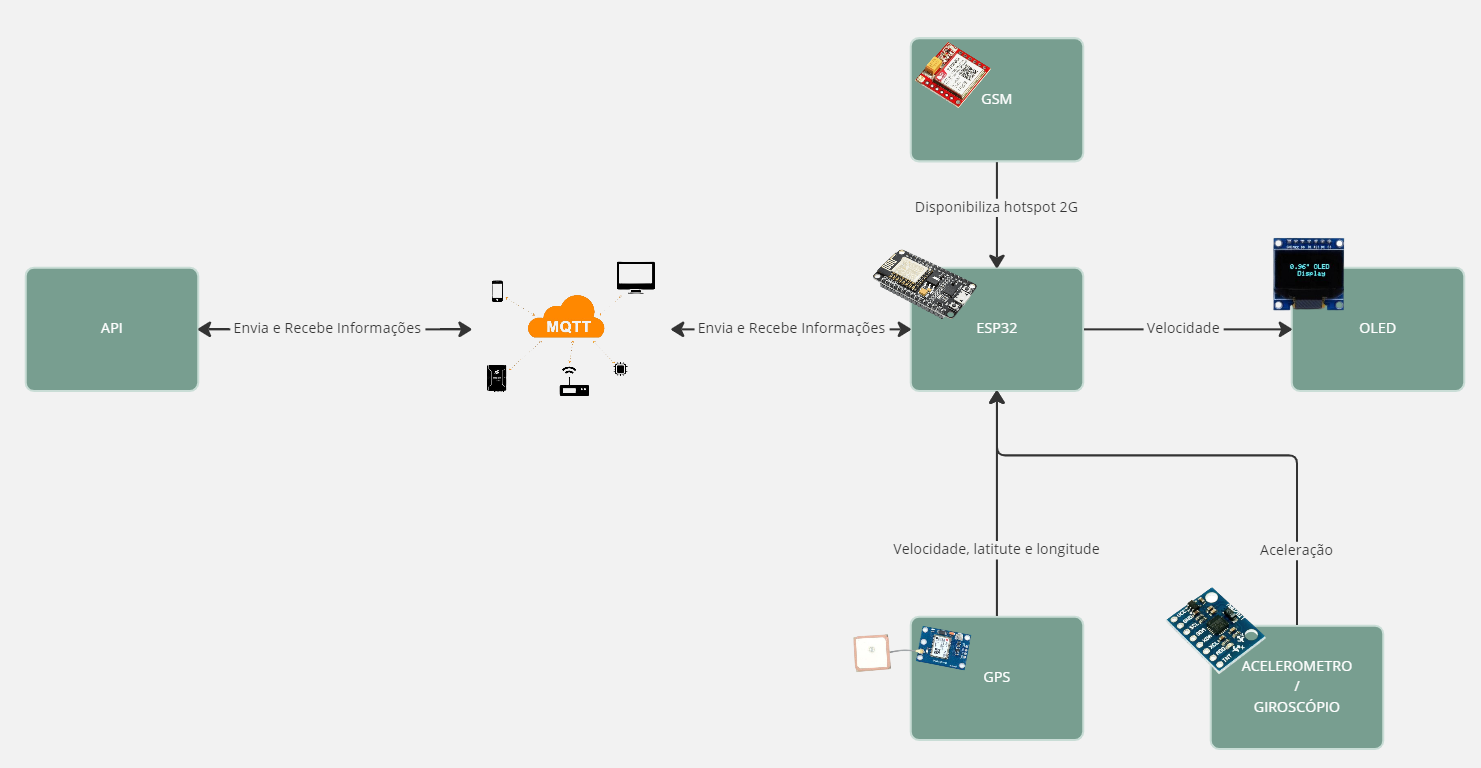
\includegraphics[width=15cm]{capitulos/Figuras/Diagrama_Hardware.png}
\caption{Diagrama geral do Projeto}
\label{fig:diagrama_hardware}
\end{figure} 

\section{Projeto mecânico}
\begin{figure}[!h]
\centering
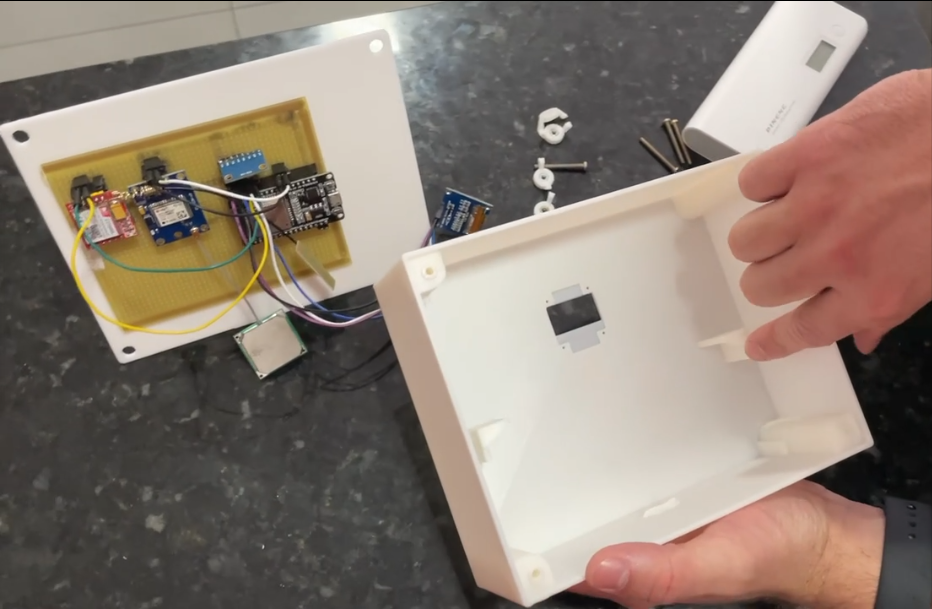
\includegraphics[width=15cm]{capitulos/Figuras/Mecanica.png}
\caption{Parte mecânica do projeto}
\label{fig:diagrama_hardware}
\end{figure}

Sobre a parte mecânica do projeto, esta foi feita quase que inteiramente por impressão 3D, usando PLA, como demonstrado nas Figuras \ref{fig:3d1} e \ref{fig:3d2}. Optou-se por utilizar o PLA devido ao seu baixo custo, mas acabamento e resistência satisfatórias. Assim, pode-se dividir o projeto em duas grandes partes mecânicas: a base do circuito com o suporte para fixação na bicicleta, e a tampa superior com um furo para posicionamento, exibição e fixação do display OLED.

Além disso, uma variável importante a se considerar na impressão 3D é o fluxo de polímero na ponteira. A base foi impressa com fluxo de 30 por cento, visando maior leveza e estabilidade na fixação do módulo. Já a tampa superior foi impressa com fluxo de 100 por cento, obtendo maior rigidez, robustez e opacidade, em detrimento da leveza.

\newpage

\begin{figure}[!h]
\centering
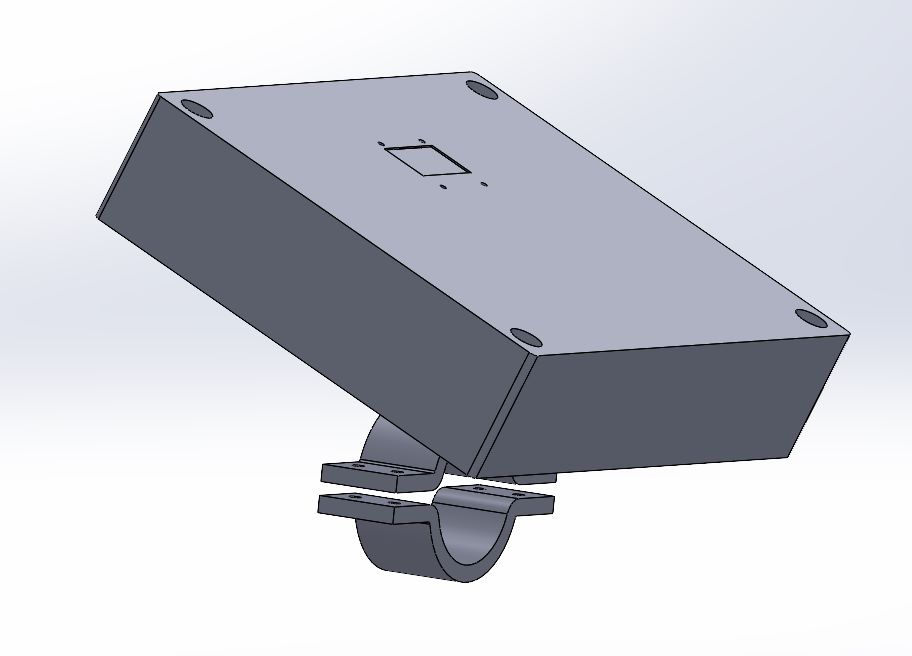
\includegraphics[width=13cm]{capitulos/Figuras/3d-1.jpg}
\caption{Visão isométrica do projeto 3D}
\label{fig:3d1}
\end{figure}

\begin{figure}[!h]
\centering
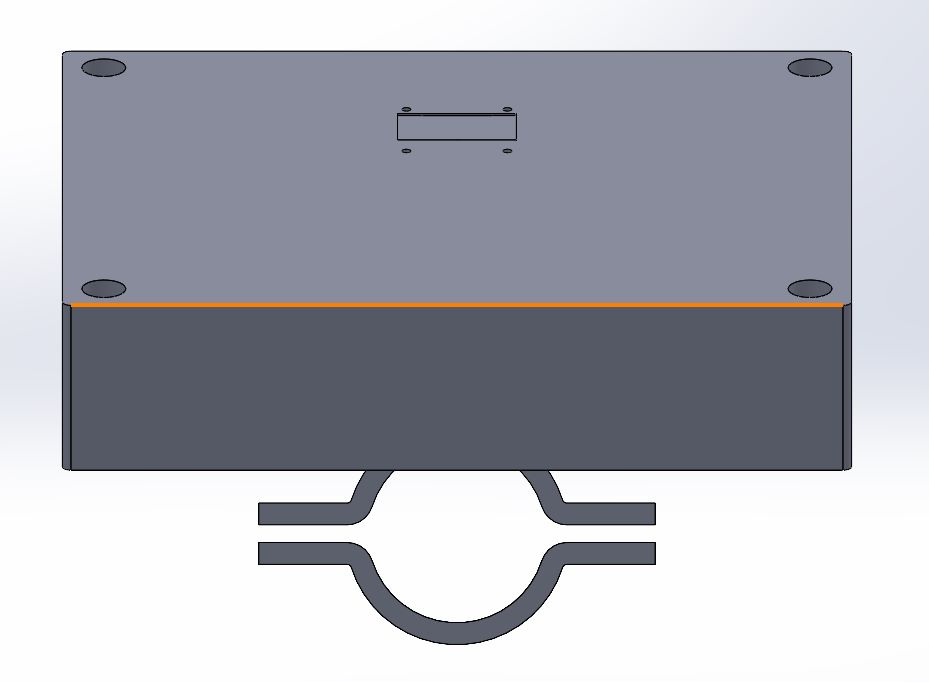
\includegraphics[width=13cm]{capitulos/Figuras/3d-2.jpg}
\caption{Visão frontal do projeto 3D}
\label{fig:3d2}
\end{figure}

\newpage
Em paralelo, foram impressas borboletas para envolver as porcas do projeto, a fim de auxiliar o usuário na fixação, desafixação e abertura do módulo quando necessário. Foram utilizados então parafusos e porcas avulsos, para fixação e ajuste do módulo.

Subsequentemente, foram realizados testes e experimentos a fim de validar a resistência do conjunto, com acelerações, movimentos bruscos e vibrações. Em todos os testes a montagem desempenhou muito bem, em nenhum momento deslizando ou abrindo demasiadamente.

\newpage
\section{Projeto de hardware}

Abaixo na Figura \ref{fig:diagrama_hardware} é possivel verificar um esquematico geral do projeto com o ESP32, GPS, OLED, acelerometro, GSM e a bateria de 7.4V.
\begin{figure}[!h]
\centering
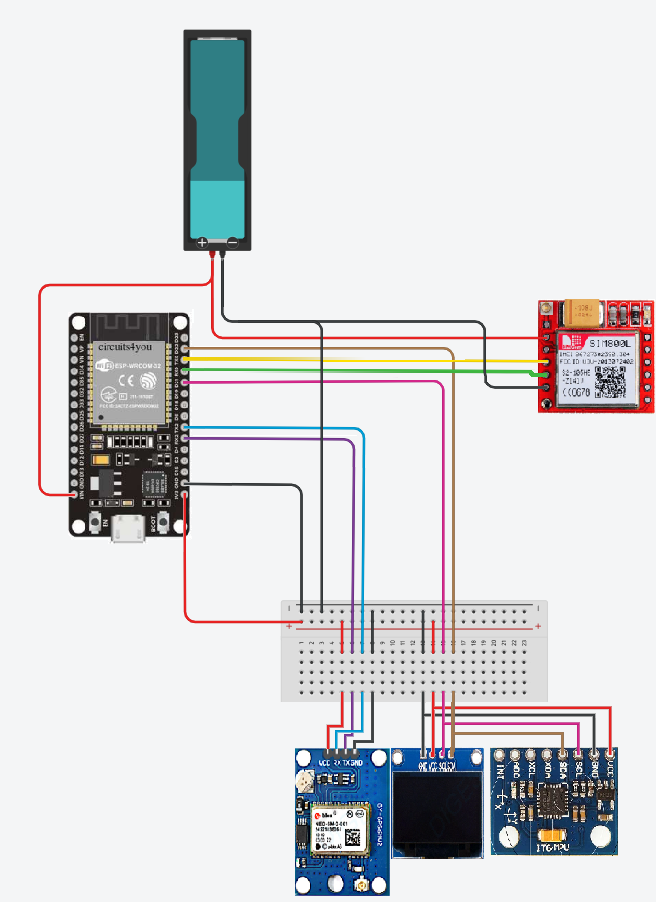
\includegraphics[width=15cm, height=20cm]{capitulos/Figuras/Circuito.png}
\caption{Circuito do projeto}
\label{fig:diagrama_hardware}
\end{figure}

\newpage
\section{Projeto de software}

O software do projeto é constituído em três partes, o software do microcontrolador, da API, e do aplicativo Android. Porém, para uma melhor explicação será apresentado o conjunto desses três componentes.

A comunicação Módulo-API é feita através de um broker MQTT da HiveMQ, para essa comunicação existem 4 tópicos. O ESP32 faz subscribe no tópico /bike/park (para receber o pedido de estacionar), e de forma contrária a API faz publish nesse tópico. O ESP32 também faz subscribe nos tópicos /bike/location (para enviar latitude, longitude e velocidade), /bike/warning (para avisar que a bicicleta saiu do lugar quando estacionada) e /bike/warning/state (para mostrar o estado atual da bicicleta, estacionada ou não), como demonstrado na Figura \ref{fig:mqtt_api_modulo}.

\begin{figure}[!h]
\centering
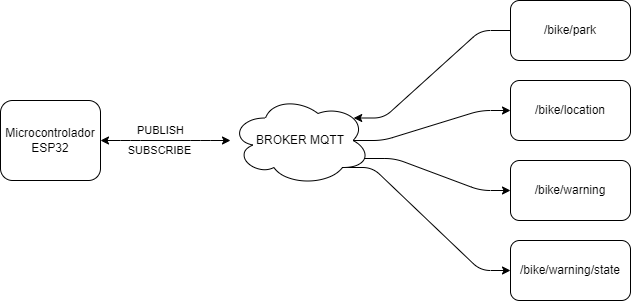
\includegraphics[width=15cm]{capitulos/Figuras/api-modulo.png}
\caption{Diagrama de comunicação ESP32-API via MQTT.}
\label{fig:mqtt_api_modulo}
\end{figure}

\newpage

A comunicação API-Aplicativo é feita de duas formas, uma via HTTP e outra via Firebase., demonstrados nas figuras \ref{fig:api_app_firebase} e \ref{fig:api_app_http}. Na comunicação via HTTP é feito um GET na rota /bike/lastLocation da API, assim retornando o último registro da latitude, longitude e velocidade da bicicleta.

\begin{figure}[!h]
\centering
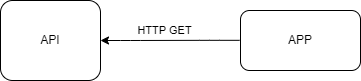
\includegraphics[width=10cm]{capitulos/Figuras/api-app.png}
\caption{Diagrama de comunicação API-Aplicativo via HTTP.}
\label{fig:api_app_firebase}
\end{figure}

\begin{figure}[!h]
\centering
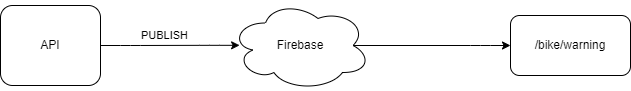
\includegraphics[width=15cm]{capitulos/Figuras/api-firebase.png}
\caption{Diagrama de comunicação API-Aplicativo via Firebase.}
\label{fig:api_app_http}
\end{figure}

Para o funcionamento do estacionamento da bicicleta, que é a ativação do modo de segurança da bicicleta, demonstrado na Figura \ref{fig:park-bike}. O fluxo começa com o usuário apertando o botão de estacionamento no aplicativo, que por sua vez envia um HTTP POST para a API, após isso é enviado um publish no /bike/park via MQTT e recebido no ESP32, após isso é desligado a tela OLED. Enquanto o modo estacionar estiver ligado o ESP32 irá monitorar o acelerômetro, e caso haja movimento (sendo um possível roubo) é enviado um MQTT publish para o tópico /bike/warning, que é recebido pela API e depois enviada para o aplicativo via Firebase. O fluxo termina com o usuário desativando o modo de estacionamento (caso não tenha sido ativado o \textit{warning}), que por sua vez envia um HTTP POST para a API, após isso é enviado um publish no /bike/park via MQTT e recebido no ESP32, após isso é ligado a tela OLED novamente, como demonstrado na Figura \ref{fig:unpark-bike}.

\begin{figure}[!h]
\centering
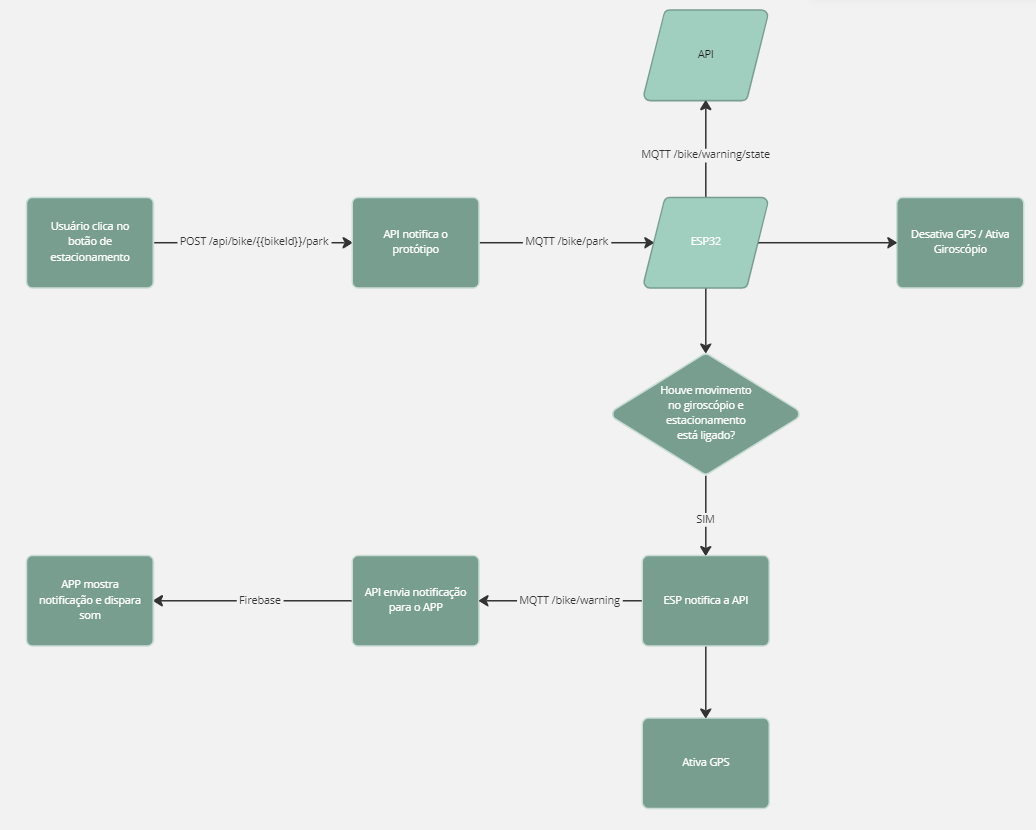
\includegraphics[width=15cm]{capitulos/Figuras/Software_Estacionar.png}
\caption{Software em modo estacionar.}
\label{fig:park-bike}
\end{figure}

\begin{figure}[!h]
\centering
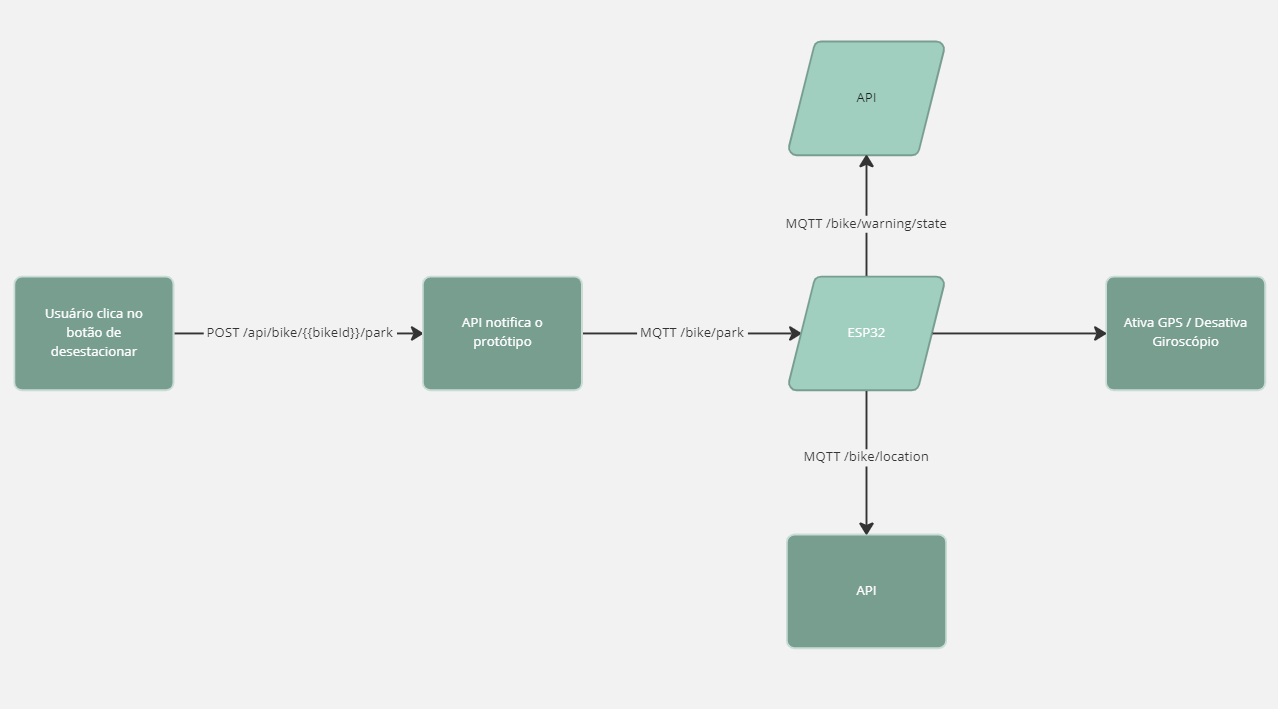
\includegraphics[width=15cm]{capitulos/Figuras/Software_Desestacionar.png}
\caption{Software em modo desestacionar.}
\label{fig:unpark-bike}
\end{figure}

\newpage
\section{Integração}
Por fim, a integração das fontes foi através de protocolos MQTT e HTTP. Por consequência, poucas mudanças basais no projeto ocorreram a partir de problemas de integração, as mudanças foram exclusivamente relacionadas com problemas de hardware, descritos com maior ênfase no tópico subsequente.   %Metodologia
\chapter{Experimentos e resultados}
Em linhas gerais, a maior parte do desenvolvimento das frentes de mecânica do projeto se deram de forma tranquila e progressiva, bem como o desenvolvimento do software. A impressão 3D aconteceu de forma planejada e cadenciada, com grande enfoque no desenho e modelagem antes da prototipagem e testes de resistência. 

O desenvolvimento do software também correu bem, na medida do possível, visto que os integrantes do grupo já haviam tido contato com as tecnologias utilizadas na disciplina de Oficina de Integração 1, portanto não ocorreram grandes surpresas no desenvolvimento desta parte do projeto.

Os maiores problemas e consequentes gargalos ocorreram na parte de hardware, com componentes estragando ou não funcionando conforme o esperado sendo os principais destes problemas:
    
\begin{itemize}
  \item GPS com problema: impactou nos testes de hardware fez com que todos demorassem consideravelmente mais, pois era necessário iniciar o cold start do GPS devido a um problema interno em sua bateria.
  \item Segundo GPS com problema: observando os problemas do primeiro GPS, foi comprado um segundo GPS para substituir o antigo, porém este também veio com defeito e não funcionou conforme o esperado, forçando com que fosse utilizado o primeiro novamente.
  \item Bateria com corrente baixa: impactou nos testes do GSM, não conseguimos fazê-lo funcionar pois a corrente fornecida pela bateria era abaixo da mínima requerida pelo GSM. A bateria gerava 800mA e seria necessário no mínimo 1.5A.
  \item Problemas com o powerbank: planejou-se utilizar o powerbank para substituir a bateria pois ele tem uma saida de 5V com 2A, o que em teoria seria o suficiente para todo o projeto. Porém, realizou-se testes e o powerbank não foi suficiente para alimentar o ESP e o GSM, pois continuava não fornecendo energia suficiente.
  \item Queima do OLED: durante a fase final do projeto o OLED queimou e parou de funcionar, assim sendo necessário comprar um novo para a substituição à tempo da entrega.
  \item Possível problema com o Step Down LM2596: durante a fase final do projeto, foi comprada uma fonte de 12V e 10A para alimentar o GSM. O plano era usar o step down para abaixar essa tensao para 4.4V, porém mesmo com essa configuração não foi possivel testar o funcionamento. Outro teste foi realizado utilizando uma fonte regulável da UTFPR e com isso foi possível testar o GSM. Portanto, suspeita-se que o step down estaria prejudicando o funcionamento do GSM.
\end{itemize}

Considerando todas as falhas que ocorreram no projeto, em especial aquelas que envolveram o GSM, optou-se por substituí-lo por Hotspot 4G de um celular Android, visto que a lógica do funcionamento permaneceria coerente. Infelizmente o ESP32 trabalha com redes de 2.4GHz somente, e com celulares Apple isto não seria possível.

Ademais, a integração deu-se baseada sempre em planos paralelos e decisões visando contornar os problemas encontrados na parte de hardware, visando sempre sacrificar o mínimo da integridade e qualidade do projeto possível, mantendo suas funcionalidades.
% testes, integração, etc.

\section{Software}
O software para a API foi desenvolvido com base no proposto para o projeto, através do NodeJS e MongoDB, onde as localizações estão sendo salvas e posteriormente acessadas, como demonstrado na Figura \ref{fig:mongodb-locations}.

\begin{figure}[!h]
\centering
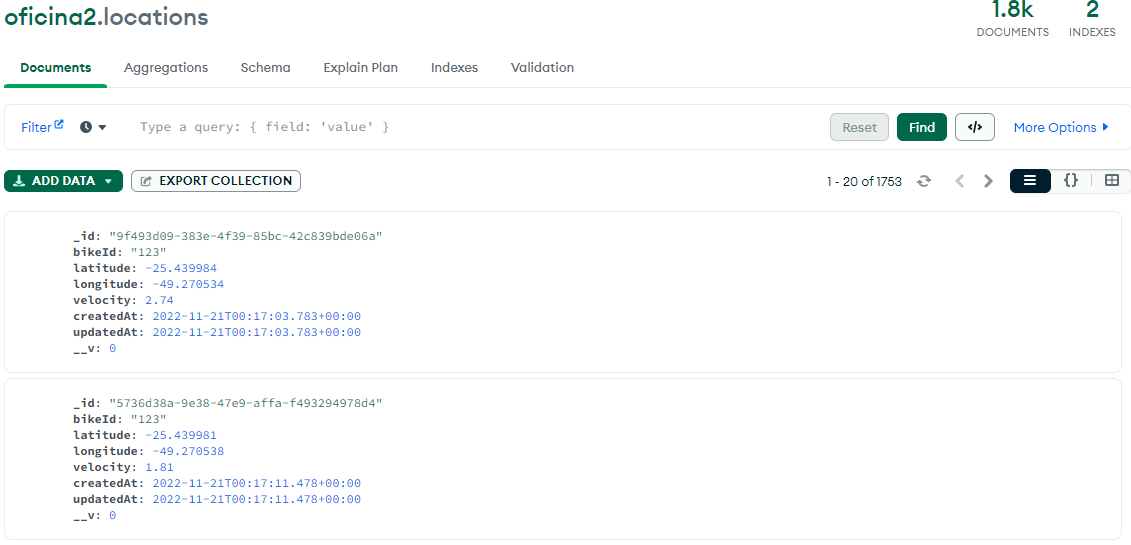
\includegraphics[width=15cm]{capitulos/Figuras/mongo-locations.png}
\caption{Localizações salvas no Banco de Dados.}
\label{fig:mongodb-locations}
\end{figure}

O software para o aplicativo também foi desenvolvido com as tecnologias propostas, através de Flutter com foco no Android. O aplicativo é constituído de um mapa com uma gaveta de navegação para poder ver as bicicletas do usuário e/ou amigo, demonstrado na Figura \ref{fig:app-map}. O dono da bicicleta tem o permissionamento para estacionar a bicicleta, permissão qual o amigo não tem, demonstrados nas Figuras \ref{fig:app-owner} e \ref{fig:app-buddy} respectivamente.

\begin{figure}[!h]
\centering
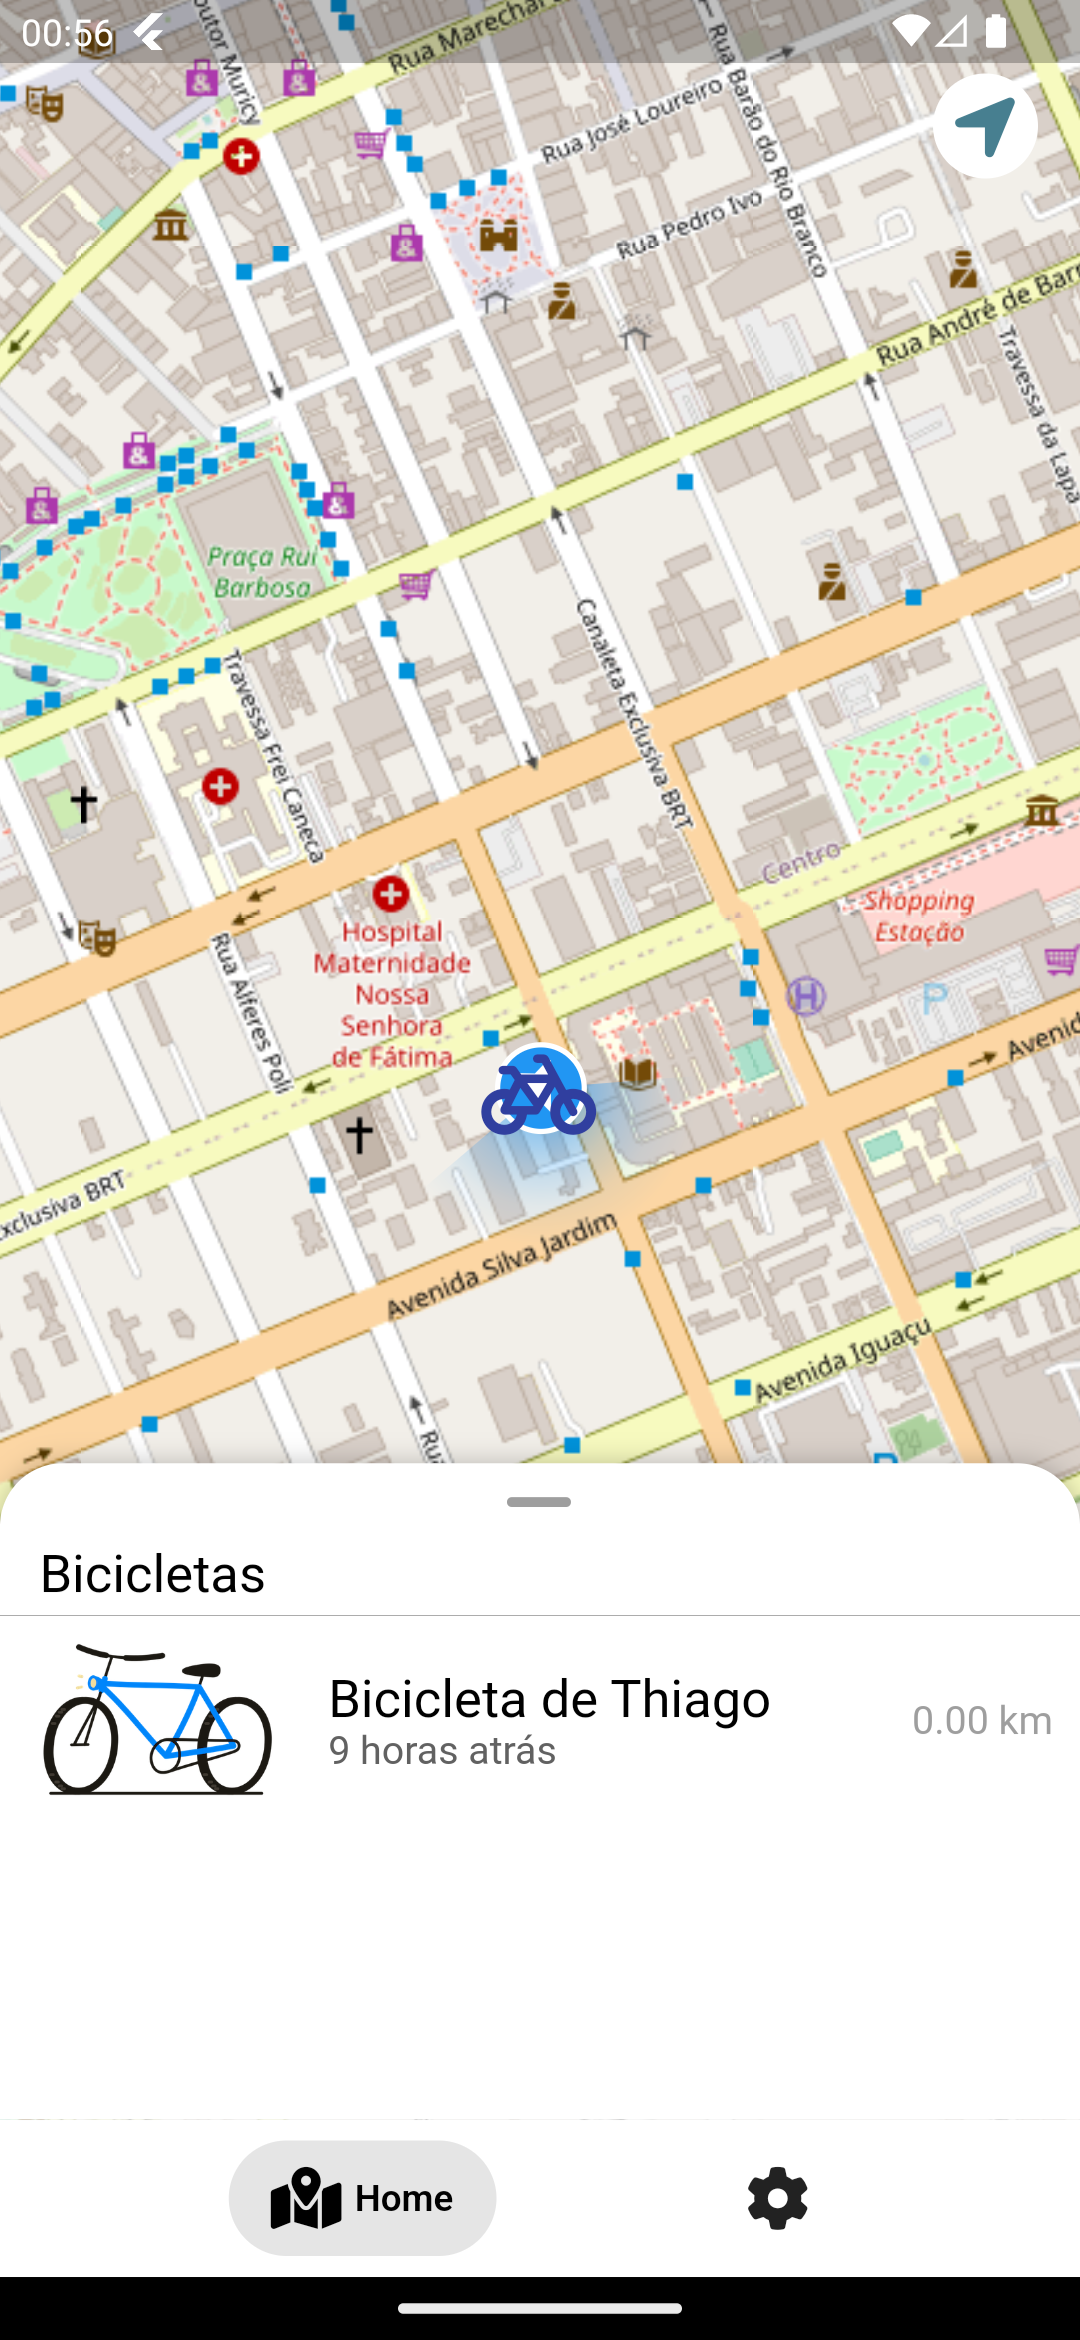
\includegraphics[width=8cm]{capitulos/Figuras/app-map.png}
\caption{Visão das bicicletas disponíveis no mapa.}
\label{fig:app-map}
\end{figure}

\newpage

\begin{figure}[!h]
\centering
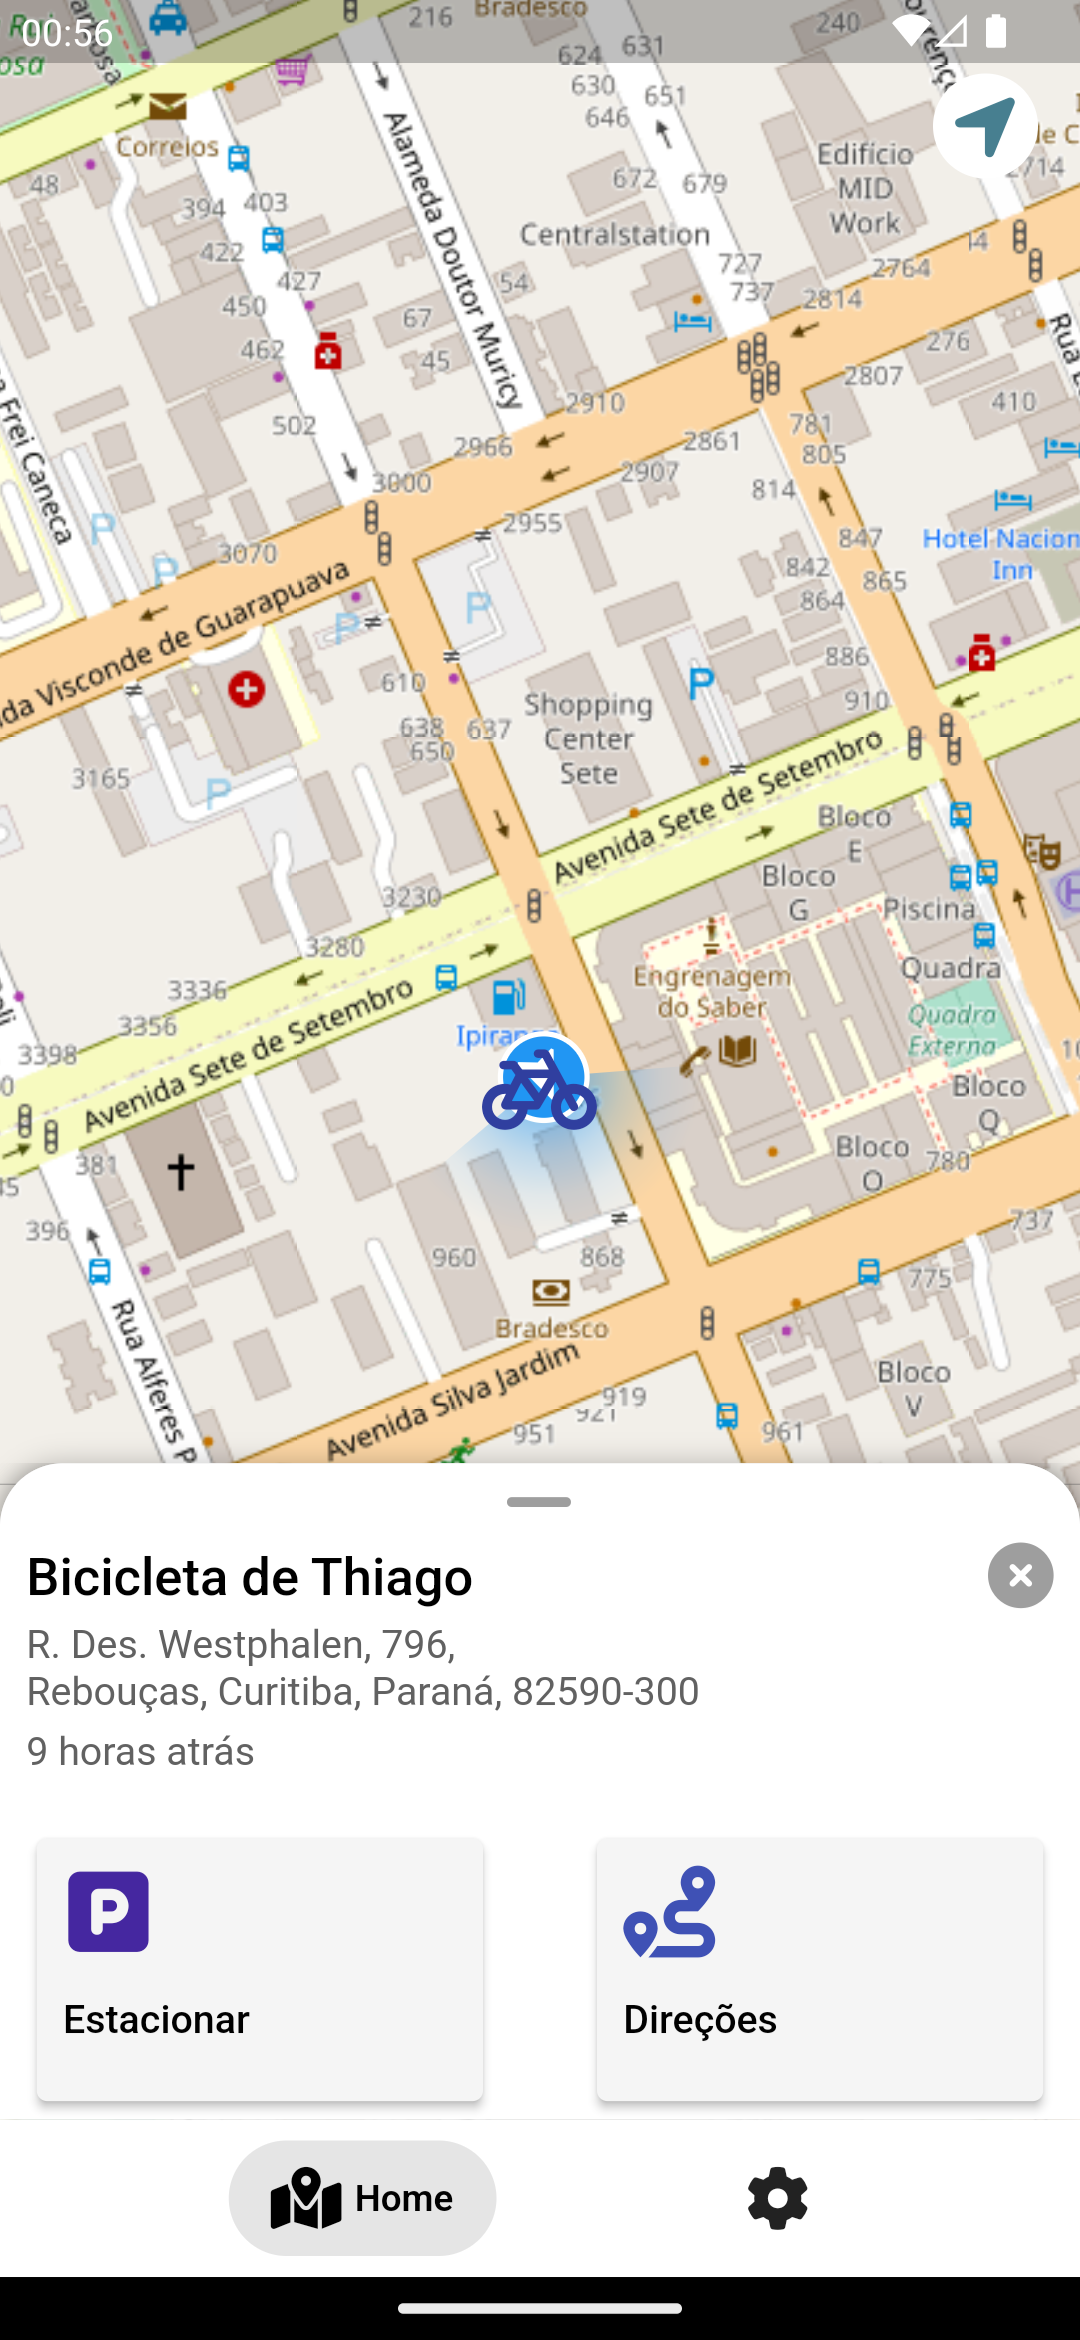
\includegraphics[width=8cm]{capitulos/Figuras/app-owner.png}
\caption{Visão do dono da bicicleta.}
\label{fig:app-owner}
\end{figure}

\newpage

\begin{figure}[!h]
\centering
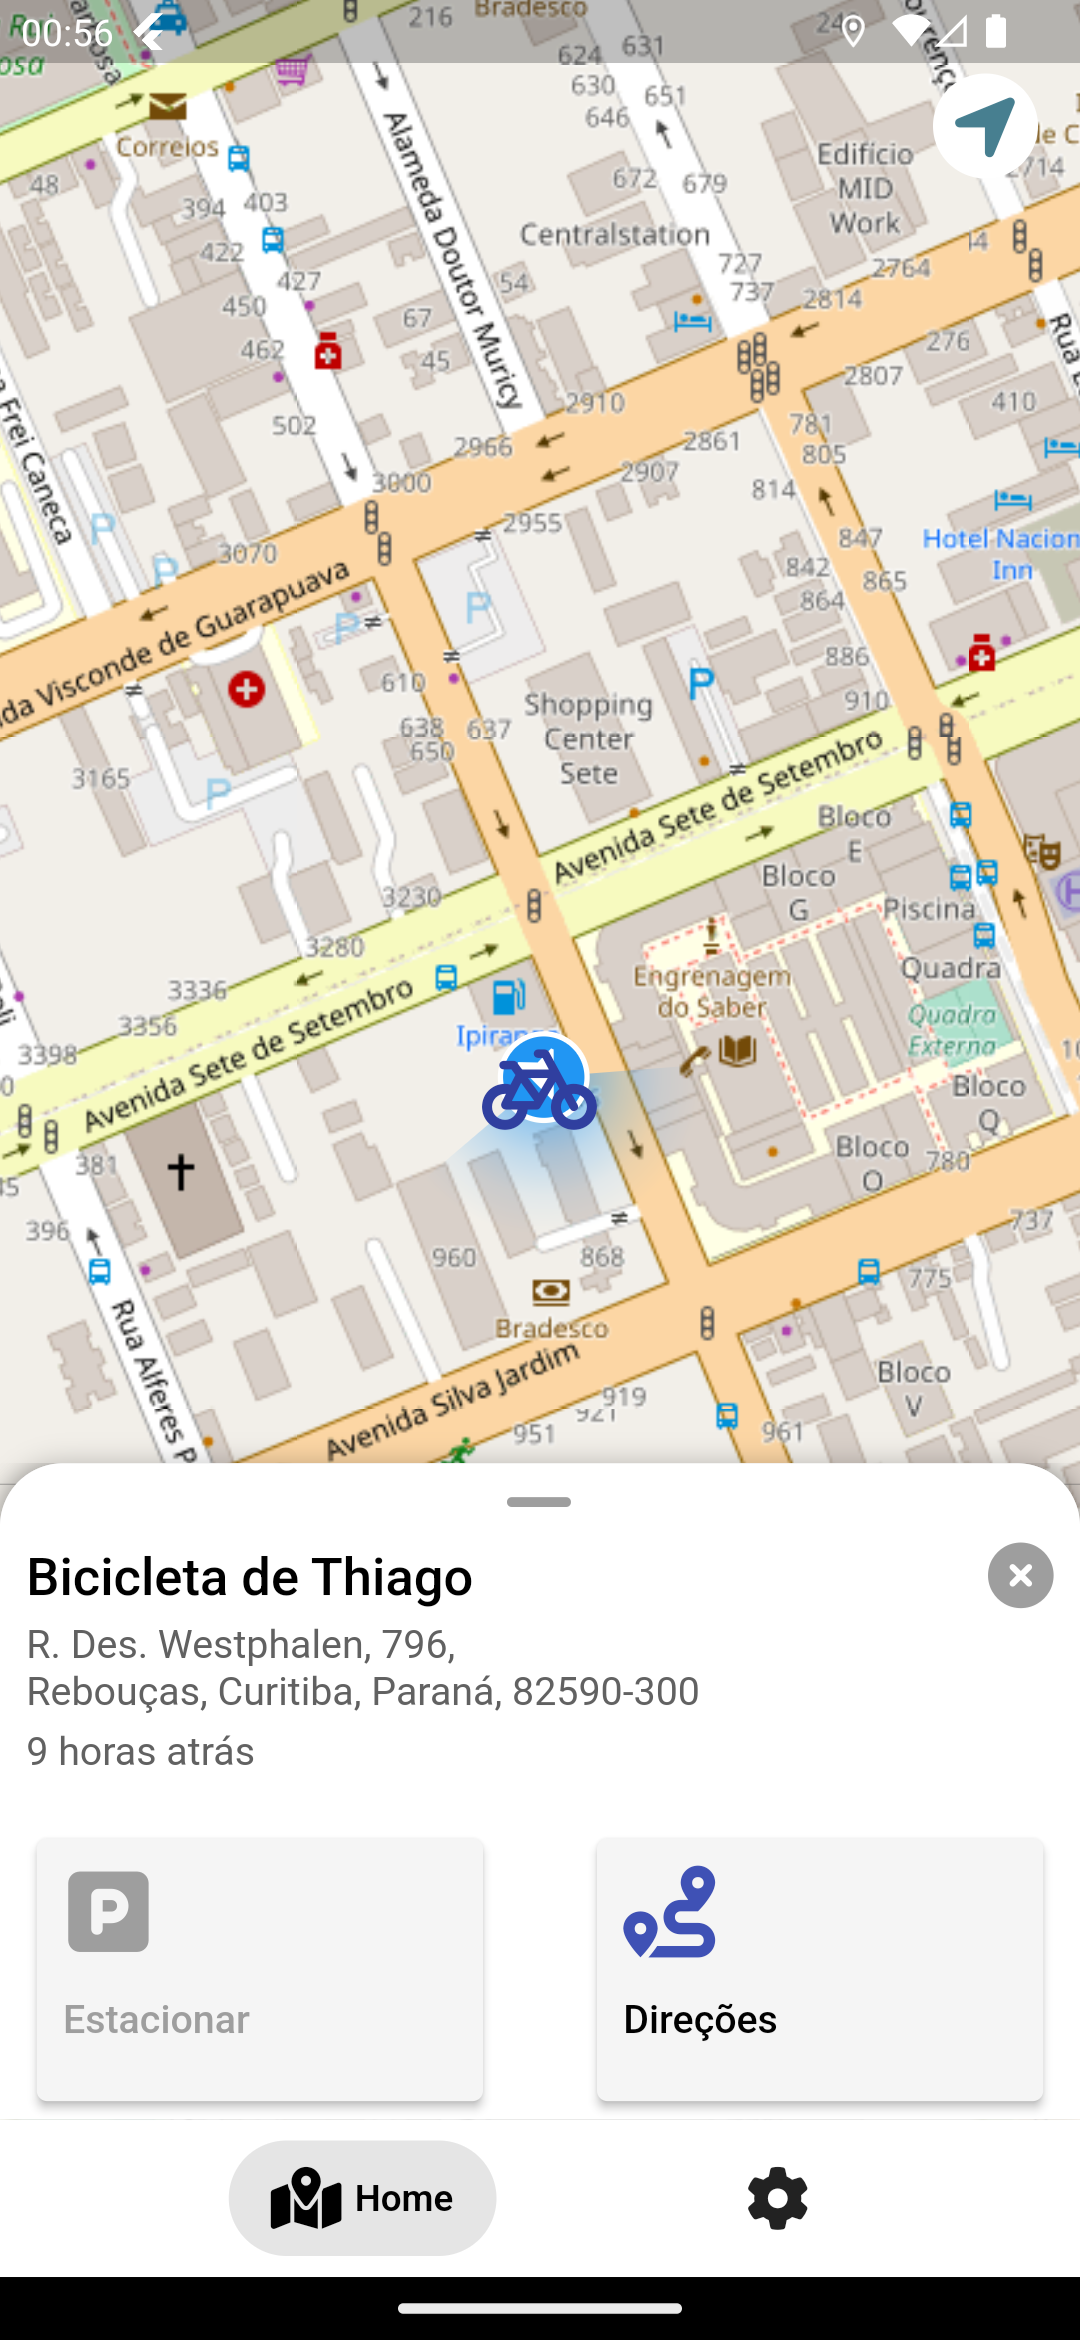
\includegraphics[width=8cm]{capitulos/Figuras/app-buddy.png}
\caption{Visão do amigo.}
\label{fig:app-buddy}
\end{figure}

\section{Hardware}

    O hardware foi montado em uma placa perfurada conforme o circuito demonstrado na Figura \ref{fig:diagrama_hardware} foi soldado diversos pinos na placa com o intuito de deixa-la modular, ou seja caso ocorra a queima de algum componente ele pode ser facilmente retirado da placa para a substituição como demonstrado na Figura \ref{fig:hardware_placa} e \ref{fig:hardware_pinos}.
    
\begin{figure}[!h]
\centering
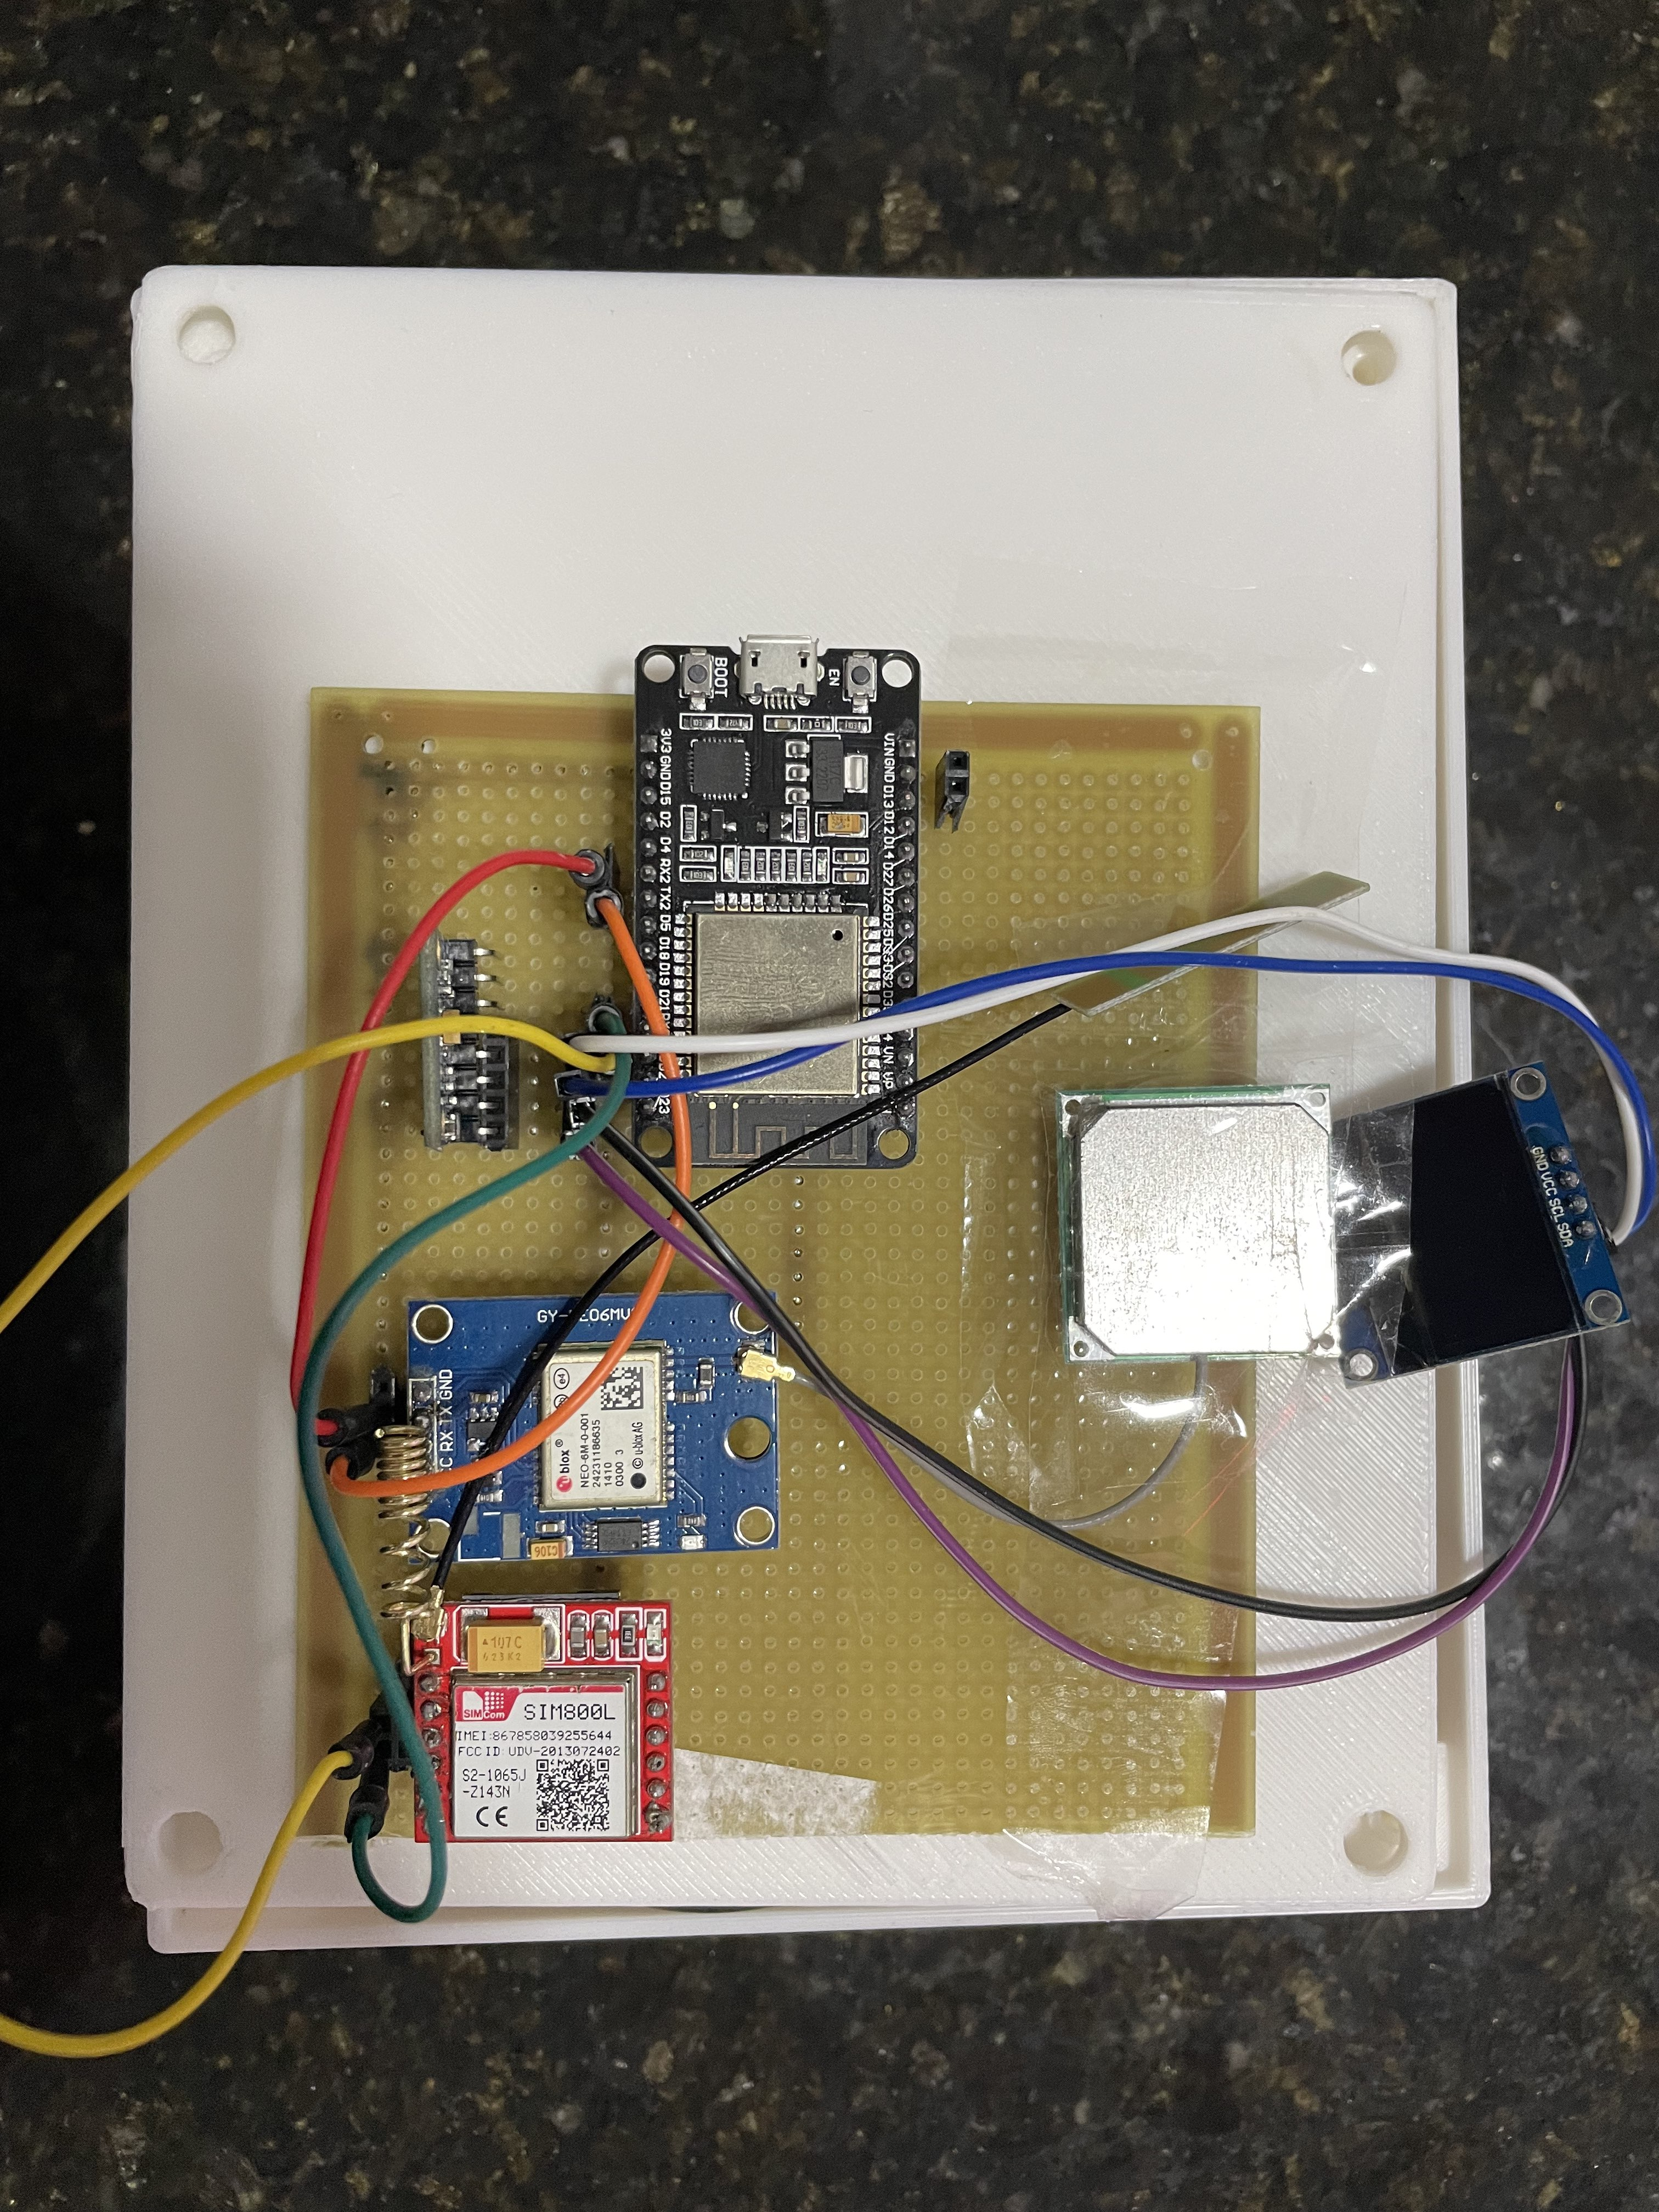
\includegraphics[width=10cm, height = 10cm]{capitulos/Figuras/Imagem_Hardware_2.jpg}
\caption{Placa perfurada.}
\label{fig:hardware_placa}
\end{figure}

\begin{figure}[!h]
\centering
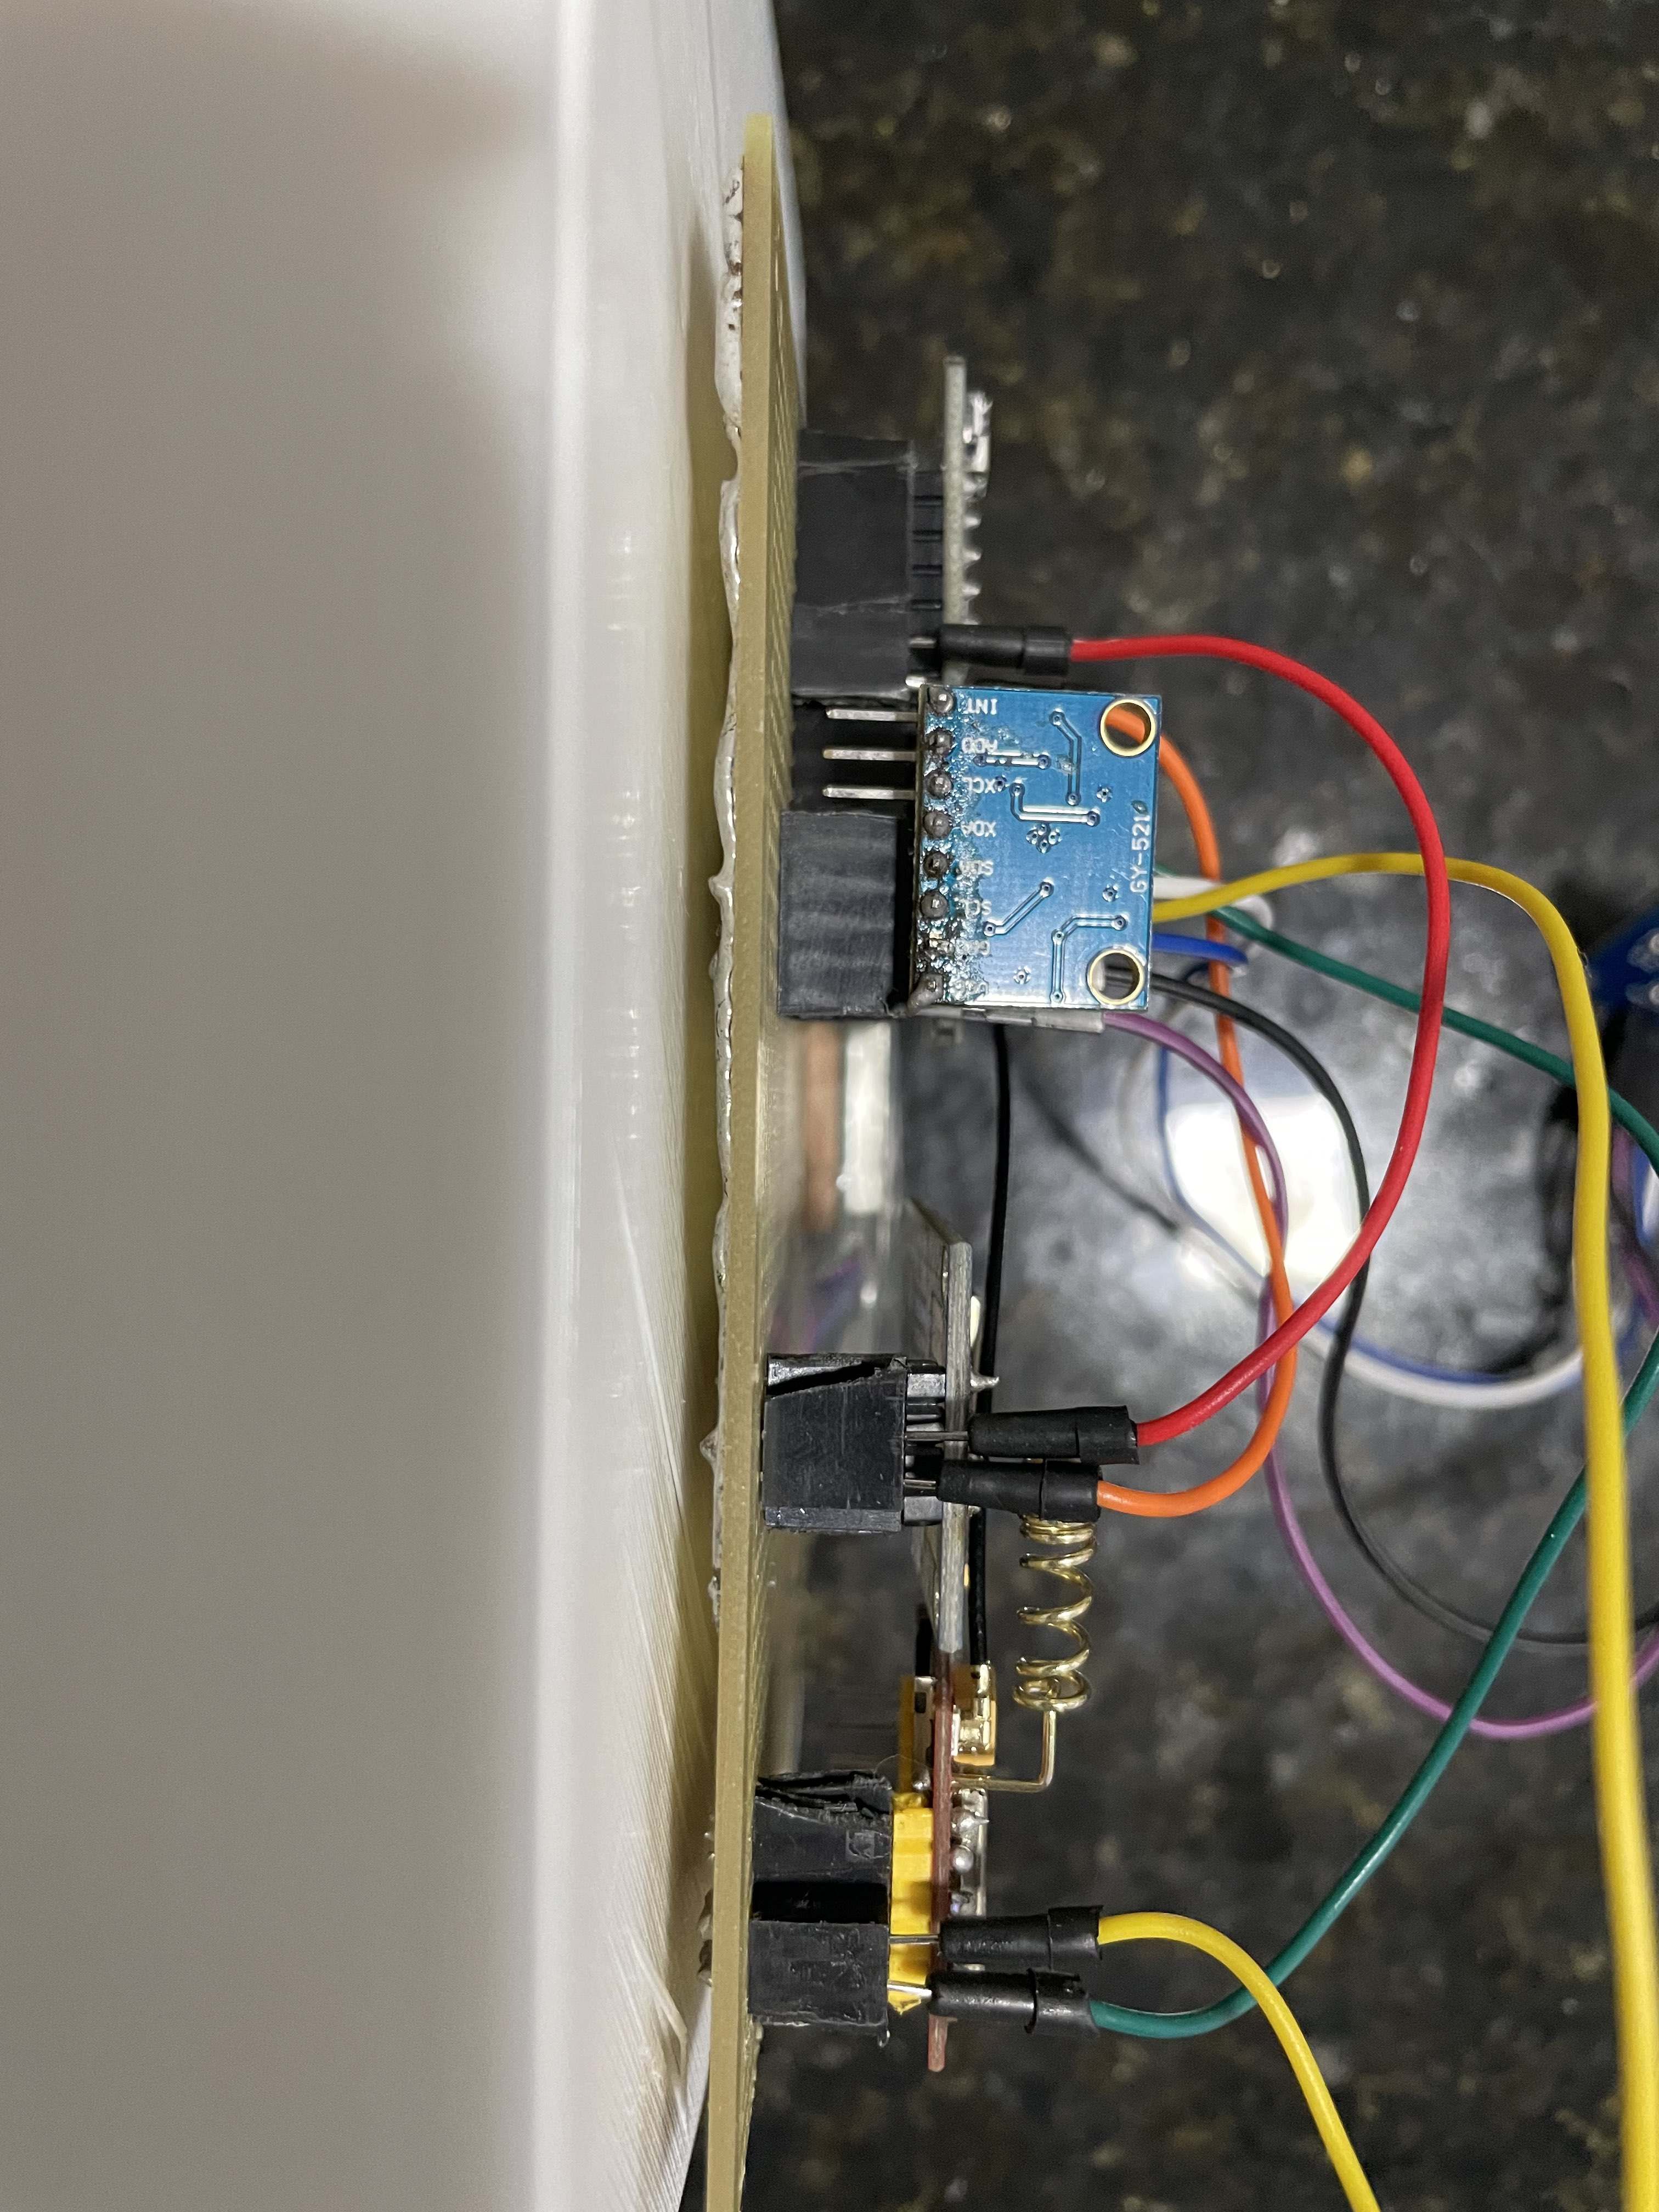
\includegraphics[width=10cm, height = 10cm]{capitulos/Figuras/Imagem_Hardware_1.jpg}
\caption{Placa perfurada pinos.}
\label{fig:hardware_pinos}
\end{figure}

   %Experimentos e resultados
\chapter{Cronograma e custos do projeto}
Um bom planejamento é essencial para o sucesso de um projeto, ainda mais quando trata-se de um trabalho em equipe. Com isso em mente, foi feito um cronograma detalhado já na proposta do GoBike, que pôde ser seguido sem grandes empecilhos, fator este que foi essencial para o sucesso do desenvolvimento. 

\section{Cronograma}

\begin{figure}[!h]
\centering
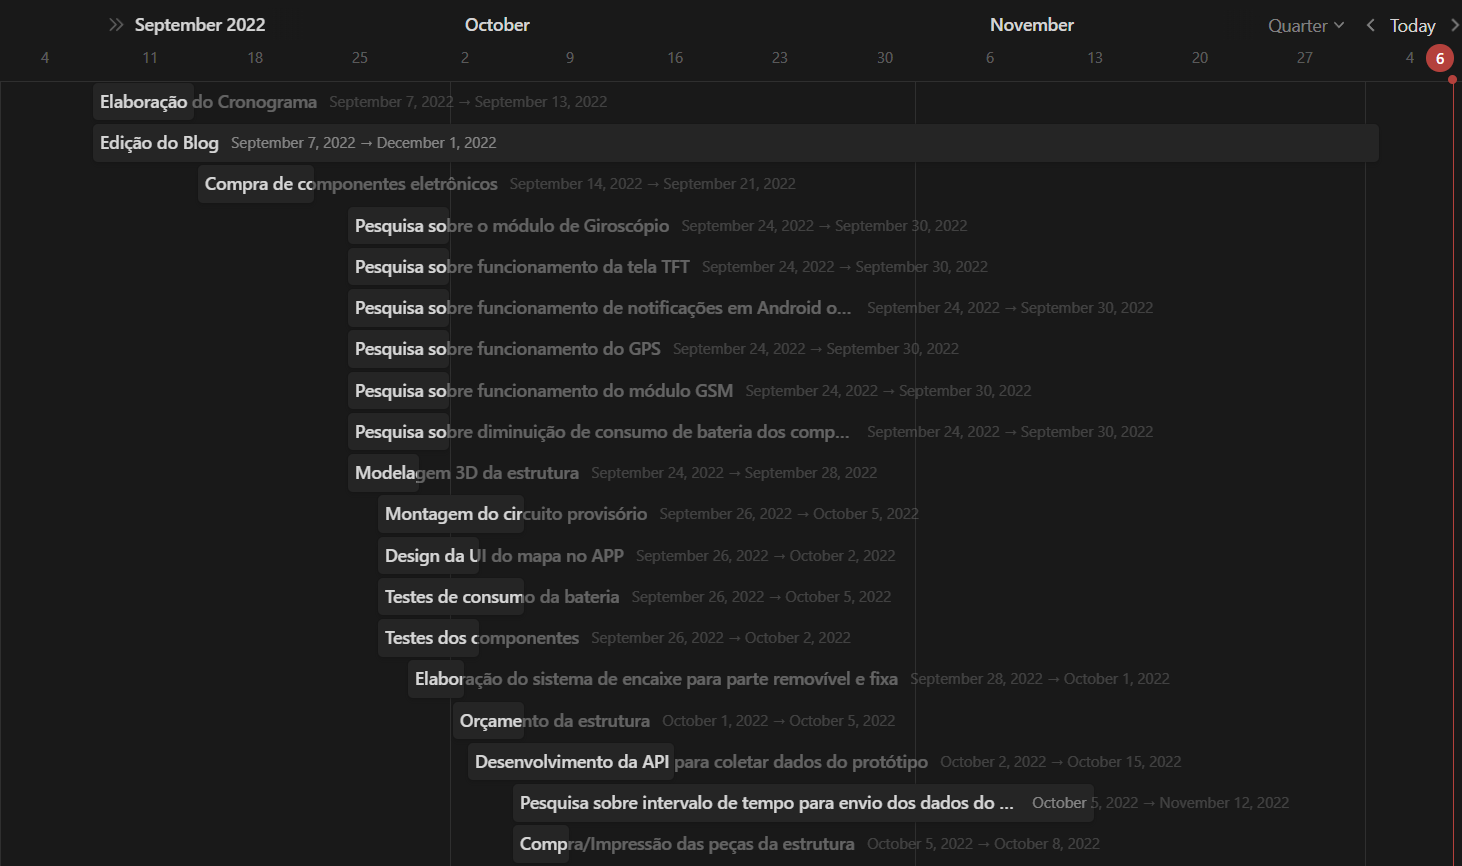
\includegraphics[width=15cm]{capitulos/Figuras/Cronograma1.png}
\caption{Cronograma do projeto (parte 1).}
\label{fig:cronograma_1}
\end{figure}

\newpage

\begin{figure}[!h]
\centering
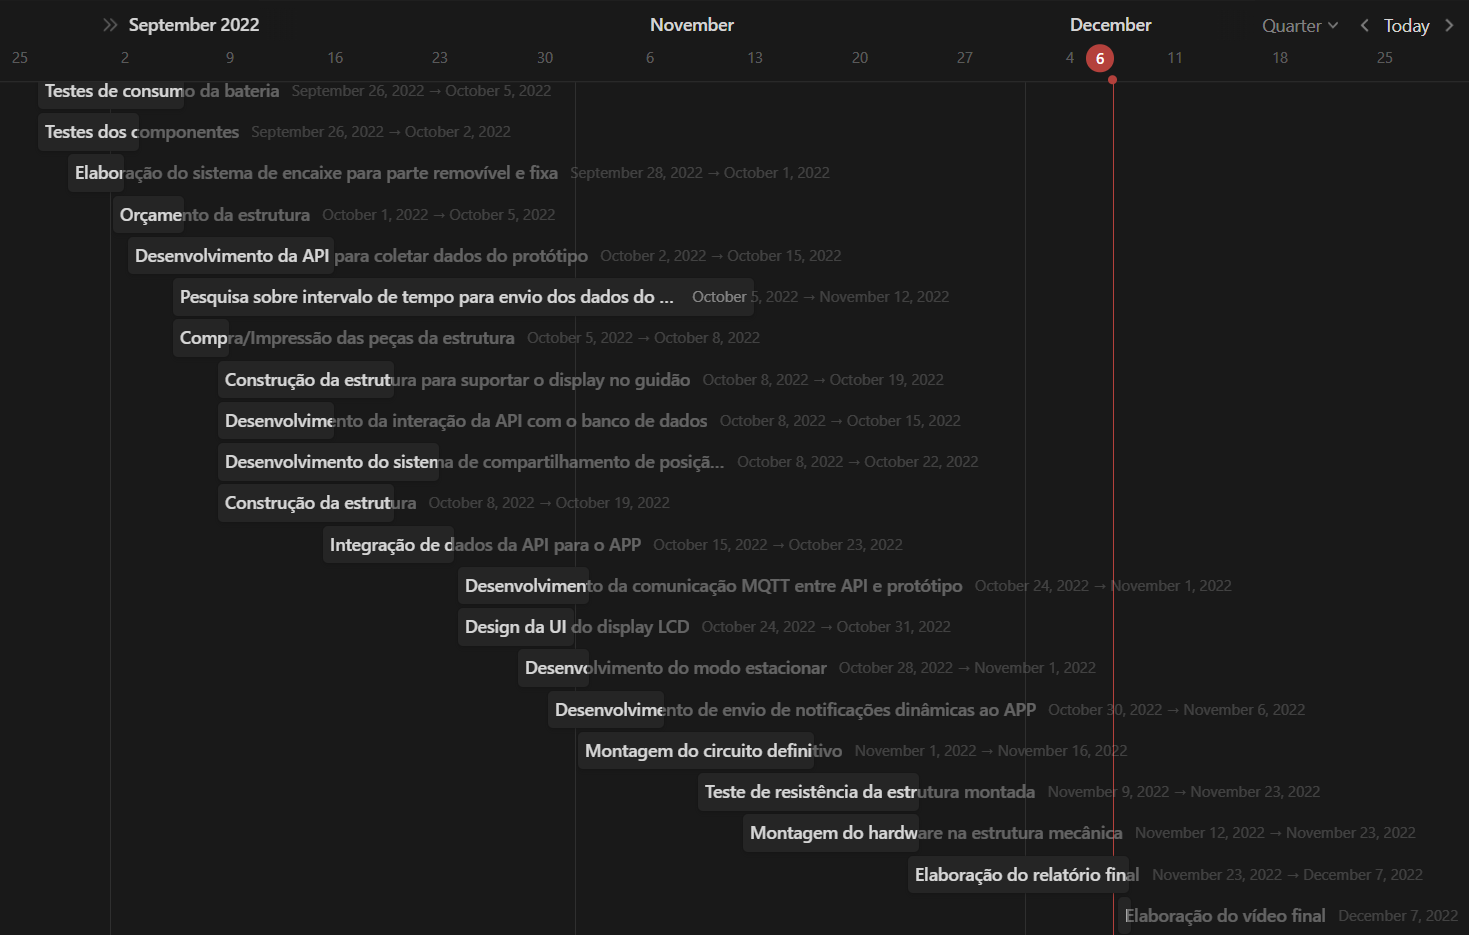
\includegraphics[width=15cm]{capitulos/Figuras/Cronograma2.png}
\caption{Cronograma do projeto (parte 2).}
\label{fig:cronograma_2}
\end{figure}

\section{Custos}

Foram desconsiderados do custo total alguns insumos básicos, como jumpers e estanho. Além disso, componentes que queimaram ou vieram com defeito também não entraram no cálculo, visto que foram imprevistos e, em condições ideais, não aconteceriam. Visto isso, o custo total estimado do projeto seria de aproximadamente R\$436,16, conforme Tabela 1 a seguir. Porém na Tabela 2 temos a lista de componentes completa, incluindo hardwares que foram comprados pra substituir os que queimaram e os que foram usados para teste e acabaram não sendo incorporados no projeto final.

\newpage

\begin{table}[]
\centering
\label{tab:componentes} 
\begin{tabular}{|l|l|l|}
\hline
Qtd. & Nome                               & Preço     \\ \hline
1    & ESP32                              & R\$72,90  \\ \hline
1    & Display OLED 0.96”                 & R\$38,61  \\ \hline
1    & Powerbank 5V 2.1A 10000 mAh        & R\$72,00  \\ \hline
1    & Módulo GSM GPRS SIM800L            & R\$ 56,90 \\ \hline
1    & Acelerômetro e Giroscópio MPU-6050 & R\$ 20,75 \\ \hline
1    & Placa Perfurada 15cmx10cm          & R\$ 10,00 \\ \hline
1    & GPS GY-NEO6MV2                         & R\$ 65,00 \\ \hline
1    & Impressão 3D                       & R\$ 100,00 \\ \hline
     & Valor Total                        & R\$ 436.16 \\ \hline
\end{tabular}
\caption{Lista de componentes}
\end{table}


\begin{table}[]
\centering
\label{tab:componentes2} 
\begin{tabular}{|l|l|l|}
\hline
Qtd. & Nome                               & Preço     \\ \hline
1    & ESP32                              & R\$72,90  \\ \hline
2    & Display OLED 0.96”                 & R\$77,22  \\ \hline
1    & Powerbank 5V 2.1A 10000 mAh        & R\$72,00  \\ \hline
1    & Módulo GSM GPRS SIM800L            & R\$ 56,90 \\ \hline
1    & Acelerômetro e Giroscópio MPU-6050 & R\$ 20,75 \\ \hline
1    & Placa Perfurada 15cmx10cm          & R\$ 10,00 \\ \hline
1    & GPS GY-NEO6MV2                        & R\$ 65,00 \\ \hline
1    & Impressão 3D                       & R\$ 100,00 \\ \hline
2    & LM2596                             & R\$ 30,00  \\ \hline
2    & MT3608                             & R\$ 30,00 \\ \hline
1    & Bateria De LiPo Recarregável 3.7V 1100mAh & R\$ 79,90 \\ \hline
1    & Carregador De Bateria LiPo         & R\$ 49,90 \\ \hline
     & Valor Total                        & R\$ 664,57 \\ \hline
\end{tabular}
\caption{Lista de componentes finais}
\end{table}   %Cronograma e custos do projeto
\chapter{Conclusões}
Sendo este um projeto com duração de um semestre, em muitos momentos o projeto estava se desenvolvendo bem, e em muitos outros não tão bem. Todo o processo de design thinking, desde a idealização até a concretização do projeto, foi feito em congruência com as demais disciplinas e demandas da faculdade, o que requeriu uma disciplina, foco e comprometimento ainda maior de toda equipe. 

\section{Conclusões}
Com o desenvolvimento deste projeto, foi possível obter diversas conclusões e aprendizados valiosos. Foram desenvolvidos e engrandecidos conhecimentos relacionados a desenvolvimento de projetos, eletrônica, programação, cronograma, soldagem, trabalho em equipe e muitos outros mais. 

Do ponto de vista do desenvolvimento, foi possível visualizar a real importância de um bom planejamento inicial, cronograma e definição do escopo do projeto. Em diversos momentos foi necessário um plano B ou até C, e a tomada de decisões rápida, diálogo e sintonia da equipe foram essenciais nestes momentos.

Por fim, sentiu-se que os pontos mais críticos do projeto foram o desenvolvimento e montagem do hardware e a integração de todas as partes. Muitas vezes, módulos que funcionavam separados não funcionaram em conjunto, e componentes paravam de funcionar de um dia para o outro, ocorridos estes que tornaram-se os maiores pontos de dificuldade do nosso projeto. Saber lidar com imprevistos, ter paciência e tomar decisões planejadas reforçaram a confiança e motivação da equipe em diversos momentos no decorrer do semestre.

\section{Trabalhos futuros}
Para futuros projetos, com certeza serão levados ainda mais em consideração os possíveis erros e problemas com hardware e integração, prevendo tempo de trabalho e opções paralelas para que estes não sejam gargalos no desenvolvimento. 

Além disso, serão levados todos os aprendizados e conhecimentos para futuros projetos, tanto profissionais quanto acadêmicos, pois a abordagem positiva para obter soluções é a melhor técnica quando se pretende desenvolver algum projeto, e neste tivemos oportunidade de exercitar e aprimorar constantemente estes conhecimentos e muitos outros mais.

%ex.: melhorias,  entre outros.   %Conclusoes e trabalhos futuros

%---------- Referencias ----------
%\clearpage % this is need for add +1 to pageref of bibstart used in 'ficha catalografica'.
%\label{bibstart}
%\bibliography{reflatex} % geracao automatica das referencias a partir do arquivo reflatex.bib
%\label{bibend}
\chapter{Referências}
Guia Completo do Display OLED – O que é? Como funciona?. Blog Eletrogate, 2021. Disponível em: https://blog.eletrogate.com/guia-completo-do-display-oled-parte-1-o-que-e-como-funciona-2/. Acesso em: 05 de dezembro de 2022.

ARQUITETURA DE TELAS TFT-LCD COM MICROCONTROLADORES E INTERFACES GRÁFICAS EM SISTEMAS EMBARCADOS. Repositório UTFPR, 2019. Disponível em: encurtador.com.br/bgosu. Acesso em: 06 de dezembro de 2022.

Guide for I2C OLED Display with Arduino. Random Nerd Tutorials, 2016. Disponível em: https://randomnerdtutorials.com/guide-for-oled-display-with-arduino/. Acesso em: 07 de dezembro de 2022.

Many different datasheets. DATAsheets, 2022. Disponível em: https://www.datasheets.com/en. Acesso em: 07 de dezembro de 2022.

Documentação Flutter Firebase, 2022. Disponível em: https://firebase.google.com/docs/flutter/setup. Acesso em: 08 de outubro de 2022.

Documentação Node JS, 2022. Disponível em: https://nodejs.org/en/docs/. Acesso em: 05 de outubro de 2022.

Documentação Express JS, 2022. Disponível em: https://expressjs.com/pt-br/. Acesso em: 05 de outubro de 2022.

Tutorial: Acelerômetro MPU6050 com Arduino, 2022. Disponível em: https://www.filipeflop.com/blog/tutorial-acelerometro-mpu6050-arduino/. Acesso em: 05 de outubro de 2014.

Módulo GSM SIM800L, 2018. Disponível em: https://portal.vidadesilicio.com.br/modulo-gsm-sim800l/. Acesso em: 21 de setembro de 2022.

GY-NEO6MV2 GPS Module Datasheet, 2022. Disponível em: https://s3-sa-east-1.amazonaws.com/multilogica-files/datasheets/GY-NEO6MV2-GPS-Module-Datasheet.pdf. Acesso em: 21 de setembro de 2022.

Arduino GY-NEO6MV2 GPS Module c/w Antenna & Flight Control EEPROM, 2022. Disponível em: https://www.epitran.it/ebayDrive/datasheet/NEO6MV2.pdf. Acesso em: 21 de setembro de 2022.

Controlando um display OLED com a biblioteca SSD1306, 2022. Disponível em: https://www.filipeflop.com/blog/controlando-um-display-oled-com-a-biblioteca-ssd1306/. Acesso em: 21 de setembro de 2022.

How to use MQTT in Node.js, 2021. Disponível em: https://www.emqx.com/en/blog/how-to-use-mqtt-in-nodejs. Acesso em: 08 de outubro de 2022.

ESP32 e MQTT DASH: controle e monitoramento através de um dashboard MQTT para Android, 2022. Disponível em: https://www.filipeflop.com/blog/esp32-e-mqtt-dashboard-android/. Acesso em: 21 de setembro de 2022.

Documentação MongoDB, 2022. Disponível em: https://www.mongodb.com/docs/. Acesso em: 21 de setembro de 2022.

Entenda o que é HTTP e o quão importante esse protocolo é para o seu site, 2022. Disponível em: https://rockcontent.com/br/blog/http/. Acesso em: 15 de novembro de 2022.


% %---------- Apendices (opcionais) ----------
% \apendice
% \chapter{Nome do Ap\^endice}

% Use o comando {\ttfamily \textbackslash apendice} e depois comandos {\ttfamily \textbackslash chapter\{\}}
% para gerar t\'itulos de ap\^en-dices.


% % ---------- Anexos (opcionais) ----------
% \anexo
% \chapter{Nome do Anexo}

% Use o comando {\ttfamily \textbackslash anexo} e depois comandos {\ttfamily \textbackslash chapter\{\}}
% para gerar t\'itulos de anexos.


% --------- Ordenacao Afabetica da Lista de siglas --------
%\textbf{* Observa\c{c}\~oes:} a ordenacao alfabetica da lista de siglas ainda nao eh realizada de forma automatica, porem
% eh possivel se de realizar isto manualmente. Duas formas:
%
% ** Primeira forma)
%    A ordenacao eh feita com o auxilio do comando 'sort', disponivel em qualquer
% sistema Linux e UNIX, e tambem em sistemas Windows se instalado o coreutils (http://gnuwin32.sourceforge.net/packages/coreutils.htm)
% comandos para compilar e ordenar, supondo que seu arquivo se chame 'dissertacao.tex':
%
%      $ latex dissertacao
%      $ bibtex dissertacao && latex dissertacao
%      $ latex dissertacao
%      $ sort dissertacao.lsg > dissertacao.lsg.tmp
%      $ mv dissertacao.lsg.tmp dissertacao.lsg
%      $ latex dissertacao
%      $ dvipdf dissertacao.dvi
%
%
% ** Segunda forma)
%\textbf{Sugest\~ao:} crie outro arquivo .tex para siglas e utilize o comando \sigla{sigla}{descri\c{c}\~ao}.
%Para incluir este arquivo no final do arquivo, utilize o comando \input{arquivo.tex}.
%Assim, Todas as siglas serao geradas na ultima pagina. Entao, devera excluir a ultima pagina da versao final do arquivo
% PDF do seu documento.


%-------- Citacoes ---------
% - Utilize o comando \citeonline{...} para citacoes com o seguinte formato: Autor et al. (2011).
% Este tipo de formato eh utilizado no comeco do paragrafo. P.ex.: \citeonline{autor2011}

% - Utilize o comando \cite{...} para citacoeses no meio ou final do paragrafo. P.ex.: \cite{autor2011}



%-------- Titulos com nomes cientificos (titulo, capitulos e secoes) ----------
% Regra para escrita de nomes cientificos:
% Os nomes devem ser escritos em italico, 
%a primeira letra do primeiro nome deve ser em maiusculo e o restante em minusculo (inclusive a primeira letra do segundo nome).
% VEJA os exemplos abaixo.
% 
% 1) voce nao quer que a secao fique com uppercase (caixa alta) automaticamente:
%\section[nouppercase]{\MakeUppercase{Estudo dos efeitos da radiacao ultravioleta C e TFD em celulas de} {\textit{Saccharomyces boulardii}}
%
% 2) por padrao os cases (maiusculas/minuscula) sao ajustados automaticamente, voce nao precisa usar makeuppercase e afins.
% \section{Introducao} % a introducao sera posta no texto como INTRODUCAO, automaticamente, como a norma indica.

%\balance
\end{document}
